%Time-stamp: "Last modified: 2020-09-15 16:07:32 (d_yasaki)"
\documentclass[ma]{uncgdissertationexp2}
% default is 12pt, phd, doublespaced.
% Masters students should use the ma on as shown below.
% \documentclass[ma]{uncgdissertation}

%%------------------------------------------------------------------%%
%%------------------------- Import Packages ------------------------%%
%%------------------------------------------------------------------%%
%% This is where you can put other packages that you may need. 
\usepackage{svg}
\usepackage{microtype, amsmath, amsfonts, amsthm, graphicx, booktabs}
\usepackage[colorlinks=false]{hyperref}
\usepackage[math]{blindtext} 

\usepackage[T1]{fontenc}
\usepackage{lmodern}

\usepackage[english]{babel}

\usepackage{float}

\usepackage{subcaption}
\usepackage{listings}
	\lstset{basicstyle=\ttfamily}
\usepackage{lipsum}

\usepackage{caption}
%\usepackage[svgnames]{xcolor}
%\usepackage[font={color=White},figurename=Fig.,labelfont={it}]{caption}
%%Commands definitions
%\newcommand{\setbackgroundcolor}{\pagecolor[rgb]{0,0,0}}  
%\newcommand{\settextcolor}{\color[rgb]{1,1,1}}
%\newcommand{\invertbackgroundtext}{\setbackgroundcolor\settextcolor}
%%Command execution. 
%\invertbackgroundtext


% \usepackage{showframe} 
% useful package to ensure margins are correct.
%%------------------------------------------------------------------%% 
%%--------------------------- Content ------------------------------%%
%%------------------------------------------------------------------%%
%% Members of committee.  Guidelines say don't use Dr.
%% Masters students are required to have chair plus two
%% PhD students require chair plus three.
%% The class can handle up to chair plus five.
\chair{Thomas Weighill}
\member{Michael Hull}
\member{Thomas Lewis}   
\member{MEMBER 3}   

\usepackage{graphicx}

%% Your name goes here.
% \student{Firstname}{Lastname} 
%% Some other options
\student{Sahil}{Dhawan}  % a full middle name
 
%% Thesis Title
%%    +  Capitalize first letter of important words. 
%%    +  Use inverted pyramid shape if title spans more than one line.
%%  Note: You can force break the title onto multiple lines using
%%  \break instead of \\. 
\title{Analyzing the Topological Properties of 3D STL Files}

%% Degree year.    
\degreeyear{2024}

%%------------------------------------------------------------------%% 
%%----------------------- Personal Macros --------------------------%%
%%------------------------------------------------------------------%%
%% A central location to add your favorite macros.  A few examples are
%% given below.  See tips for samples.

%% In order to get singlespacing, uncomment the line below.
%\renewcommand{\doublespacing}{\singlespacing}

%% Theorem, Lemma, etc. environments.  You can rename if you wish.                    
% Theorem style and numbering convention                                              
\theoremstyle{plain}
\newtheorem{theorem}{Theorem}[chapter]
\newtheorem{lemma}[theorem]{Lemma}
\newtheorem{proposition}[theorem]{Proposition}
\newtheorem{conjecture}[theorem]{Conjecture}
\newtheorem{corollary}[theorem]{Corollary}
\newtheorem{algorithm}[theorem]{Algorithm}

% Definition type object style and numbering convention                               
\theoremstyle{definition}
\newtheorem{definition}[theorem]{Definition}
\newtheorem{example}[theorem]{Example}

% Remark type object style and numbering                                              
\theoremstyle{remark}
\newtheorem*{remark}{Remark}  % the star makes them not numbered                      
\newtheorem*{notation}{Notation}
\newcommand{\titlecaption}[2]{\caption[#1]{#1. #2}}

%% Other macros
\newcommand{\ZZ}{\mathbb{Z}}  % Integers
\newcommand{\XX}{\mathfrak{X}}  
%%------------------------------------------------------------------%%
\pagestyle{plain} % Eliminates running headers 

\begin{document}
\frontmatter      % required

%%------------------------------------------------------------------%%
%% -------------------------- Abstract -----------------------------%%
%%------------------------------------------------------------------%%
\begin{abstract}
ABSTRACT TEXT 
\end{abstract}

%%------------------------------------------------------------------%%
%%---------------------------- Title page --------------------------%%
%%------------------------------------------------------------------%%
%% The title page is required. 
\maketitlepage  

%%------------------------------------------------------------------%%
%% ------------------------ Copyright page -------------------------%%
%%------------------------------------------------------------------%%
%% This page is required if you opt for a copyright.  Otherwise, don't
% include it.  To omit, just comment out the line below.
\makecopyrightpage

%%------------------------------------------------------------------%%
%%---------------------------- Dedication --------------------------%%
%%------------------------------------------------------------------%%
\begin{dedication}
Dedicated to my cats, Piccolo and Gohan, and my dogs, Bebe and Tilly.
\end{dedication}

%%------------------------------------------------------------------%%
%%------------------------ Approval page  --------------------------%%
%%------------------------------------------------------------------%%
%% The approval page is required.  If all of your infomation is entered
%% correctly in the contents section, this should come out correctly.
\makeapprovalpage

%%------------------------------------------------------------------%%
%%-------------------------- Acknowledgements ----------------------%%
%%------------------------------------------------------------------%%
%% The acknowledgements are optional but highly recommended.  See tips
%% for details. 
\begin{acknowledgments}
It is customary to recognize the assistance of the advisor and/or
committee chair, all other members of the committee, and only those
organizations and/or persons who actually aided the research. If
financial support was provided to make the study possible, credit for
such assistance should be given.
\end{acknowledgments}

%%------------------------------------------------------------------%%
%%----------------------------- Preface ----------------------------%%
%%------------------------------------------------------------------%%
%% The preface is optional.
\begin{preface}
A preface is a statement that either explains the author's
reasons for pursuing this subject matter or provides a personal
comment about the subject that would not otherwise be included in
the document.
\end{preface}


%%------------------------------------------------------------------%%
%%---------------------- Table of Contents -------------------------%%
%%------------------------------------------------------------------%%
%% The table of contents is required.  
\tableofcontents 

%%------------------------------------------------------------------%%
%%---------------------- List of Tables ----------------------------%%
%%------------------------------------------------------------------%%
% Recommended if you have tables.  Comment out if you don't have
% tables. 
\listoftables   


%%------------------------------------------------------------------%%
%%---------------------- List of Figures ---------------------------%%
%%------------------------------------------------------------------%%
% Recommended if you have figures.  Comment out if you don't have
% figures. 
\listoffigures   


%%------------------------------------------------------------------%%
%% This signifies that you are done with the frontmatter and ready to
%% proceed to the main part.  The rest of your document goes below.
\mainmatter % required
%%------------------------------------------------------------------%%
\chapter{Homology}

\section{Simplicial Homology}

Information in this topic is from \cite{Hatcher_2001}

A simplex is the convex hull of (n+1) points in $\mathbb{R}^{m}$ in general position.
\begin{itemize}
\item 0-simplex: a point
\item 1-simplex: an edge
\item 2-sipmlex: a "filled-in" triangle, or a triangle containing all points within the boundaries of its edges.
\item 3-simplex: a "filled-in/solid" tetrahedron, or a tetrahedron containing all points within the boundaries of its "filled-in" triangles.
\end{itemize}

\section{Persistent Homology}

\subsubsection{Cech Complexes}
$Cech_{r}(X) = \{\sigma \subseteq X \mid \cap_{x \in \sigma} B_{r}(X) \not= \emptyset\}$
\begin{itemize}
\item Balls grow around points of metric space, every time k+1 balls intersect, add a k-dimensional simplex to complex.
\end{itemize}

\subsubsection{Vietoris-Rips Complexes}
$VR_{r}(X) = \{\sigma \subseteq X \mid diam\sigma \leq 2r \}$
\begin{itemize}
\item if subsets of metric space have diameter less than or equal to 2*r, add simplex
\end{itemize}

\subsubsection{Delaunay Complexes}
$Del(X) = \{\sigma \subseteq X \mid \cap_{x \in \sigma} V_{x} \not= \emptyset\}$

$V_{x} = \{y \in \mathbb{R}^{2} \mid ||y-x|| \leq  ||y-z||, z \in X\}$
\begin{itemize}
\item Do not depend on a parameter or intersecting balls (no "time")
\item Intersecting voronoi cells determine simplices in complex
\end{itemize}

\subsubsection{Alpha Complexes}
$Alpha_{r}(X)=\{\sigma \subseteq X \mid \cap_{x\in \sigma} (B_{r}(X) \cap V_{x}) \not= \emptyset\}$
\begin{itemize}
\item in-between cech and delauney complexes: to construct, take into account both voronoi cell-associated points in metric spce and growing balls around these points
\end{itemize}

\chapter{Methods}

\section{What is an STL File?}
An STL file is 

\subsection{Converting the .ast File to a Data Structure}

The .ast file was parsed for four strings which are used to denote the beginning and end of the description of faces and vertices: "facet normal", "end facet", "outer loop", and "end loop", respectively. The data was then converted into tuple with python.

\begin{figure}[H]
\centering
% Don't indent the lstlisting environment!          
\begin{lstlisting}
solid Mesh
  facet normal 0.000000 0.000000 -1.000000
    outer loop
      vertex 4.500000 -0.288675 0.000000
      vertex 5.000000 0.577350 0.000000
      vertex 5.500000 -0.288675 0.000000
    endloop
  endfacet
  facet normal -0.816497 0.471405 0.333333
    outer loop
      vertex 5.000000 0.000000 0.816497
      vertex 5.000000 0.577350 0.000000
      vertex 4.500000 -0.288675 0.000000
    endloop
  endfacet
  facet normal 0.000000 -0.942809 0.333333
    outer loop
      vertex 5.000000 0.000000 0.816497
      vertex 4.500000 -0.288675 0.000000
      vertex 5.500000 -0.288675 0.000000
    endloop
  endfacet
  facet normal 0.816497 0.471405 0.333333
    outer loop
      vertex 5.000000 0.000000 0.816497
      vertex 5.500000 -0.288675 0.000000
      vertex 5.000000 0.577350 0.000000
    endloop
  endfacet
endsolid Mesh
\end{lstlisting}
\caption{The contents of an ASCII STL file representing a tetrahedron.}
\end{figure}
\newpage
\begin{figure}[H]
    \centering
    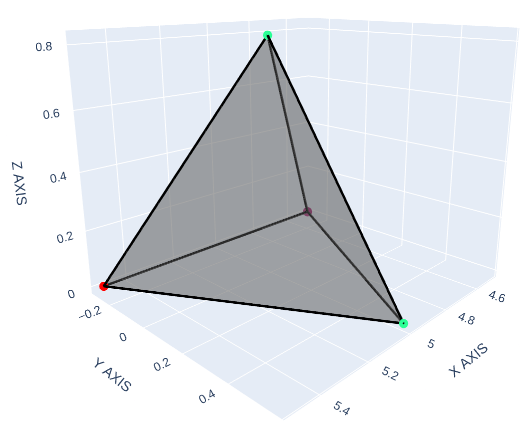
\includegraphics[width=0.5\linewidth]{tetrahedron_ast_plot.png}
    \caption{An ASCII STL file representing a tetrahedron plotted with Plotly.}
    \label{fig:ast_code}
\end{figure}

\section{Python Libraries}

\section{Meshing}

\section{Filtration Construction}

\section{Persistence Diagram Construction}

\chapter{Results}
\newpage
\begin{figure}
    \centering
    \begin{tabular}{|c|c|c|}
         \hline
         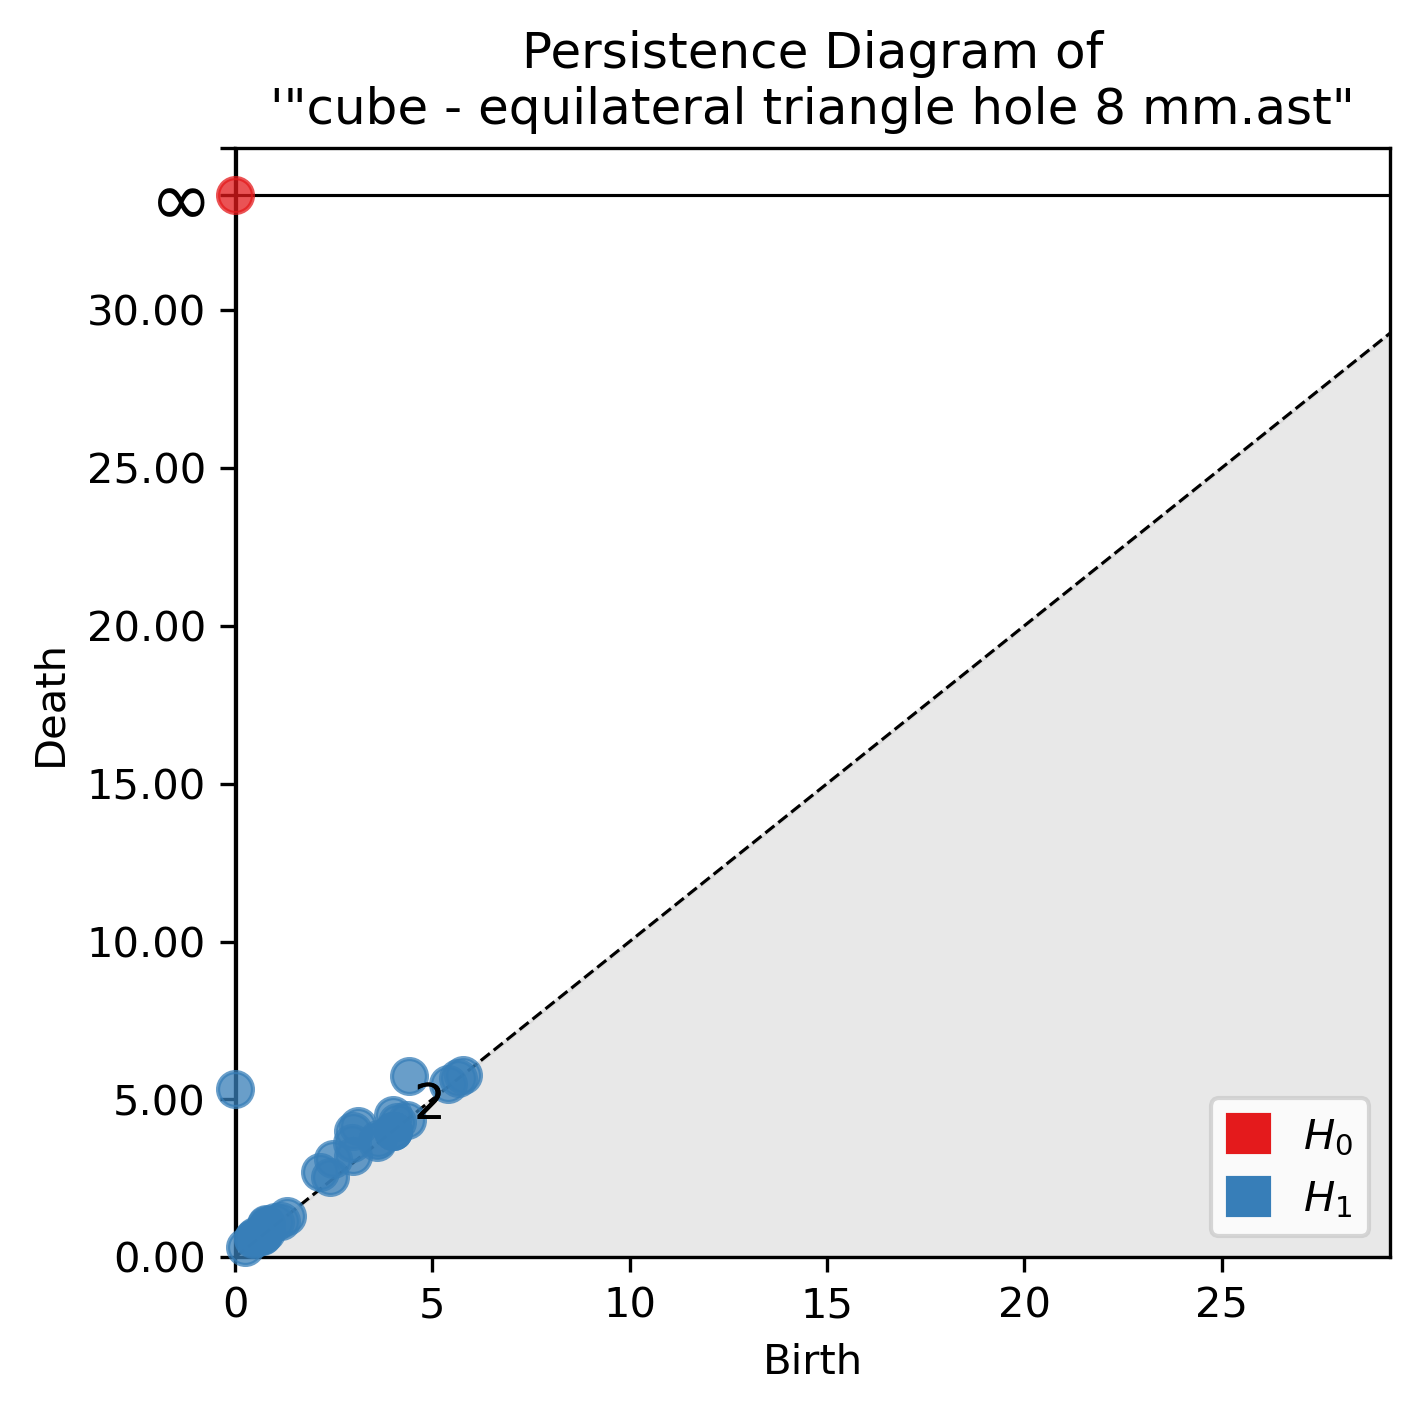
\includegraphics[width=2in]{Final Run, (cube - equilateral triangle hole 8 mm) persdia.svg} &
         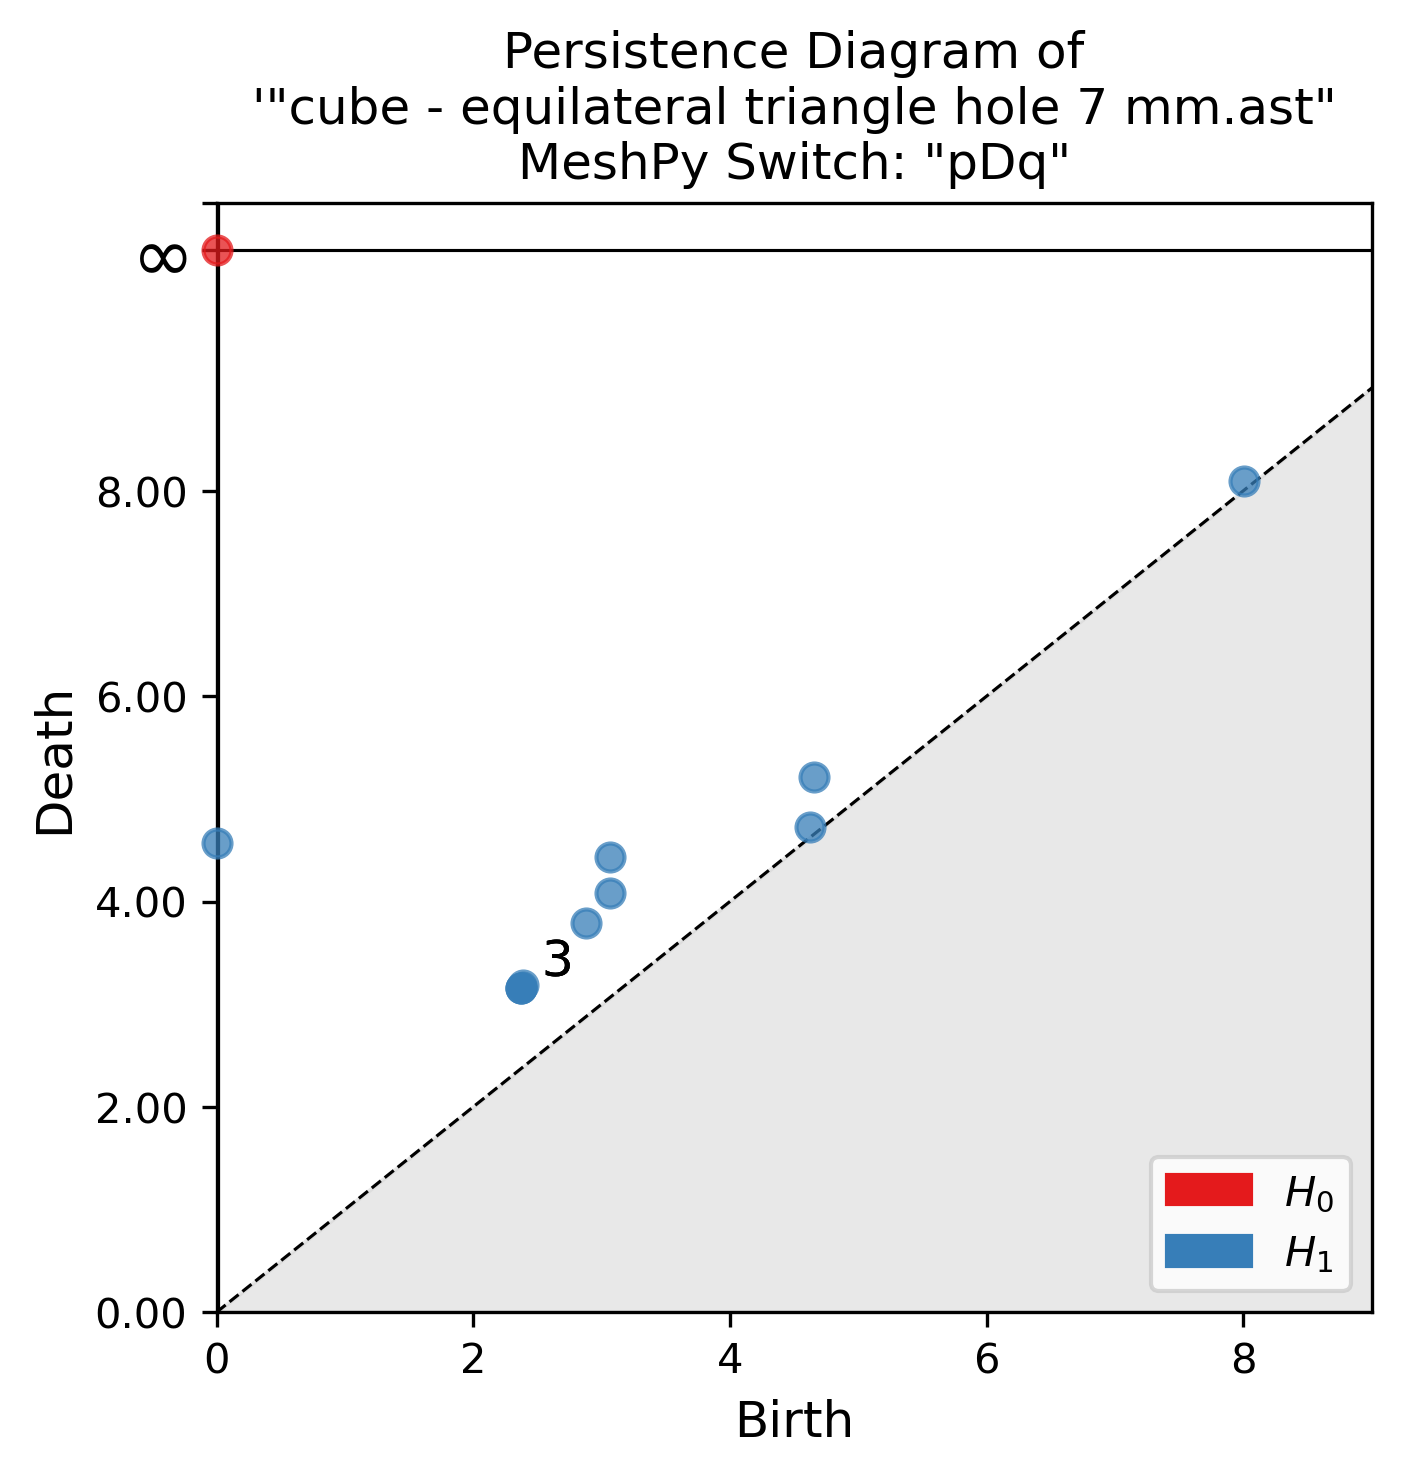
\includegraphics[width=2in]{Final Run, (cube - equilateral triangle hole 7 mm) persdia.svg} &  
         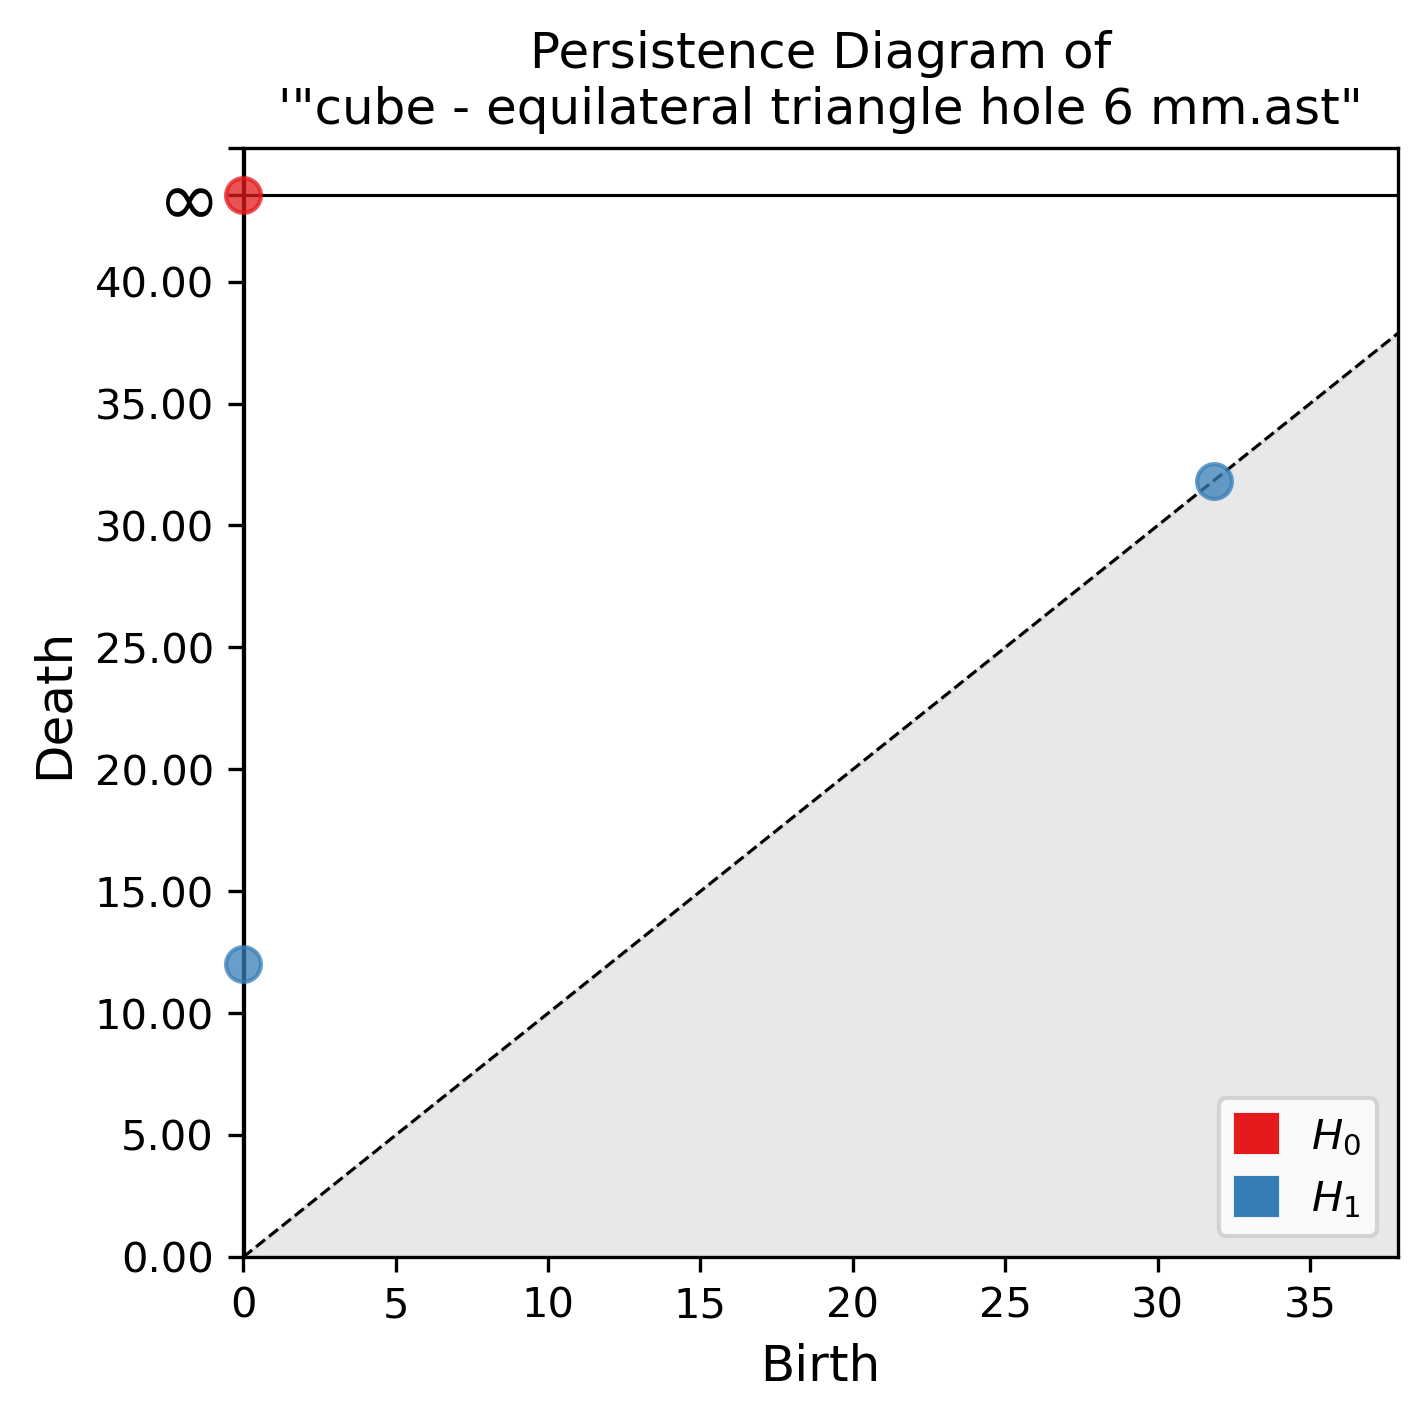
\includegraphics[width=2in]{Final Run, (cube - equilateral triangle hole 6 mm) persdia.svg} \\
         \hline
         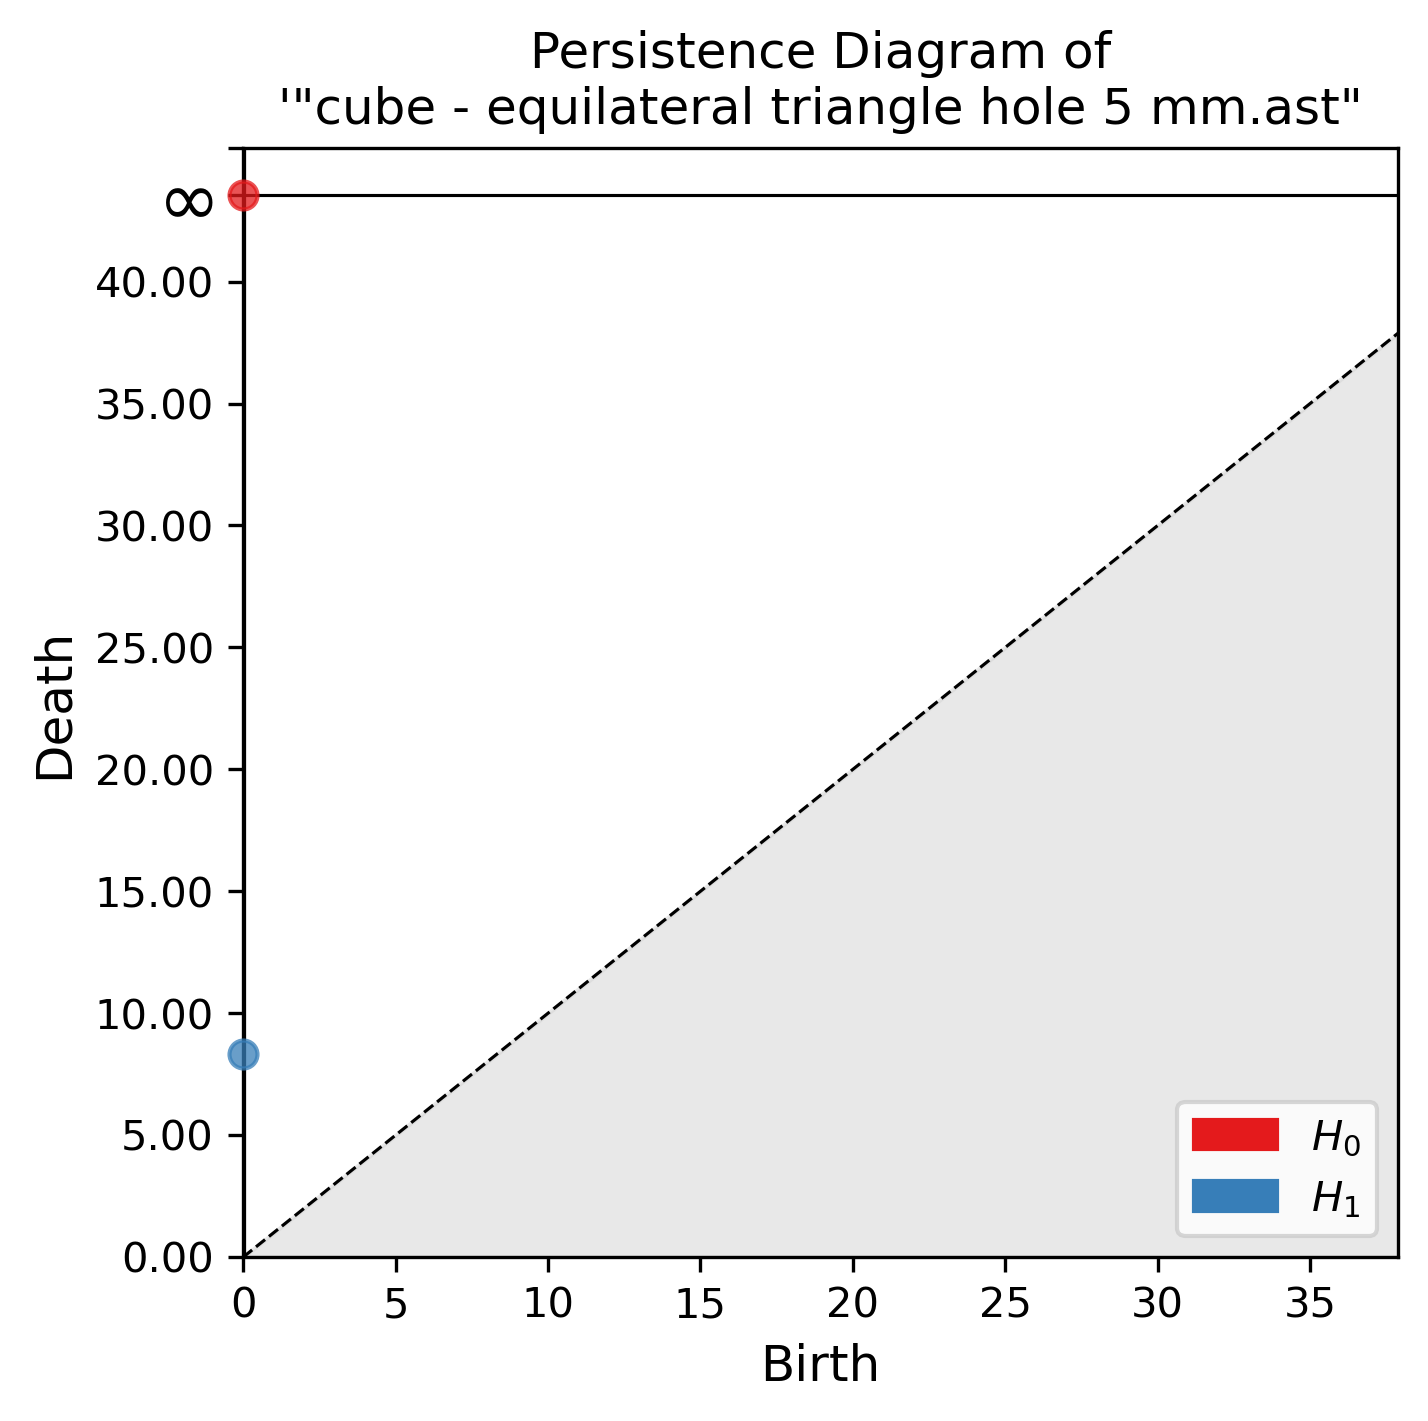
\includegraphics[width=2in]{Final Run, (cube - equilateral triangle hole 5 mm) persdia.svg} & 
         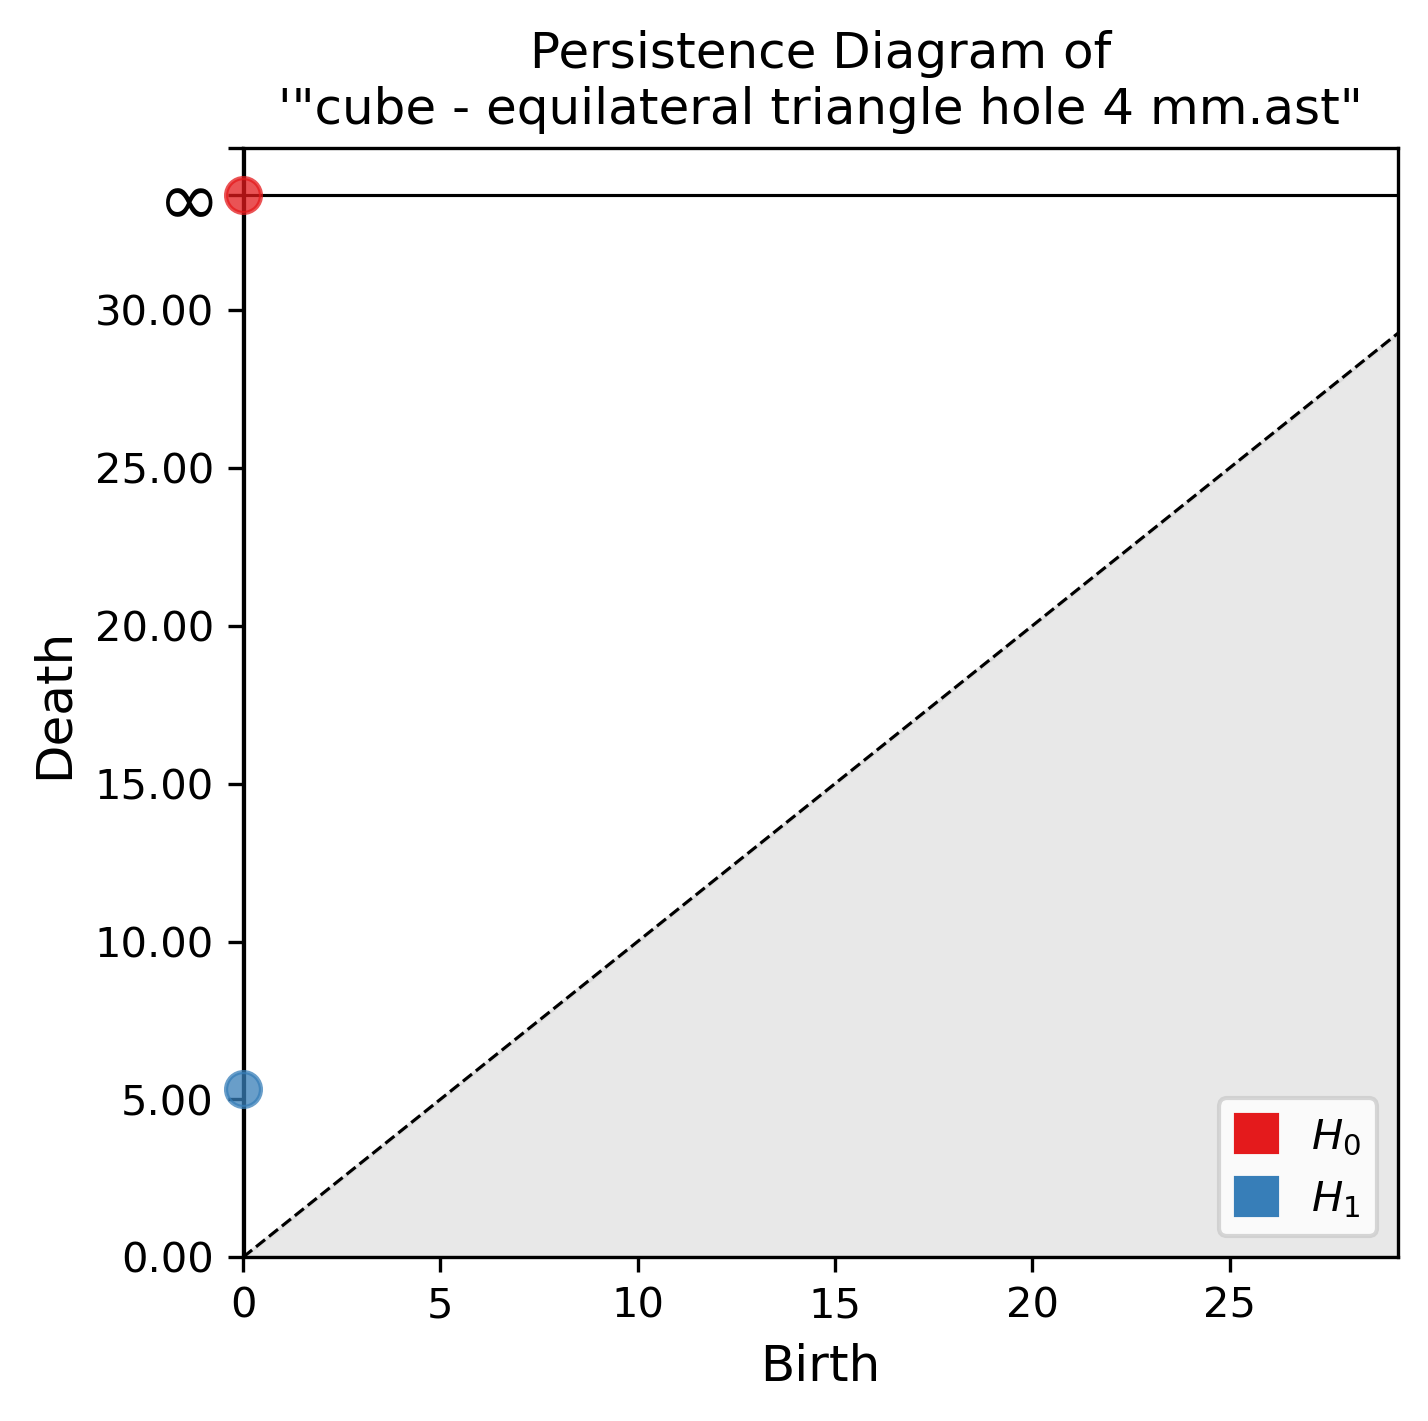
\includegraphics[width=2in]{Final Run, (cube - equilateral triangle hole 4 mm) persdia.svg} & 
         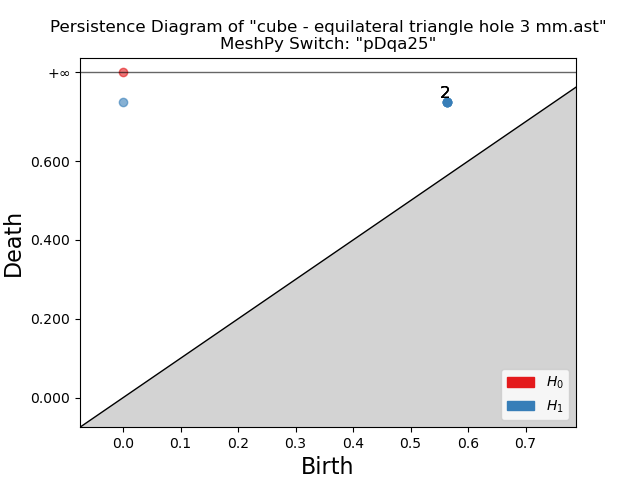
\includegraphics[width=2in]{Final Run, (cube - equilateral triangle hole 3 mm) persdia.svg} \\
         \hline
         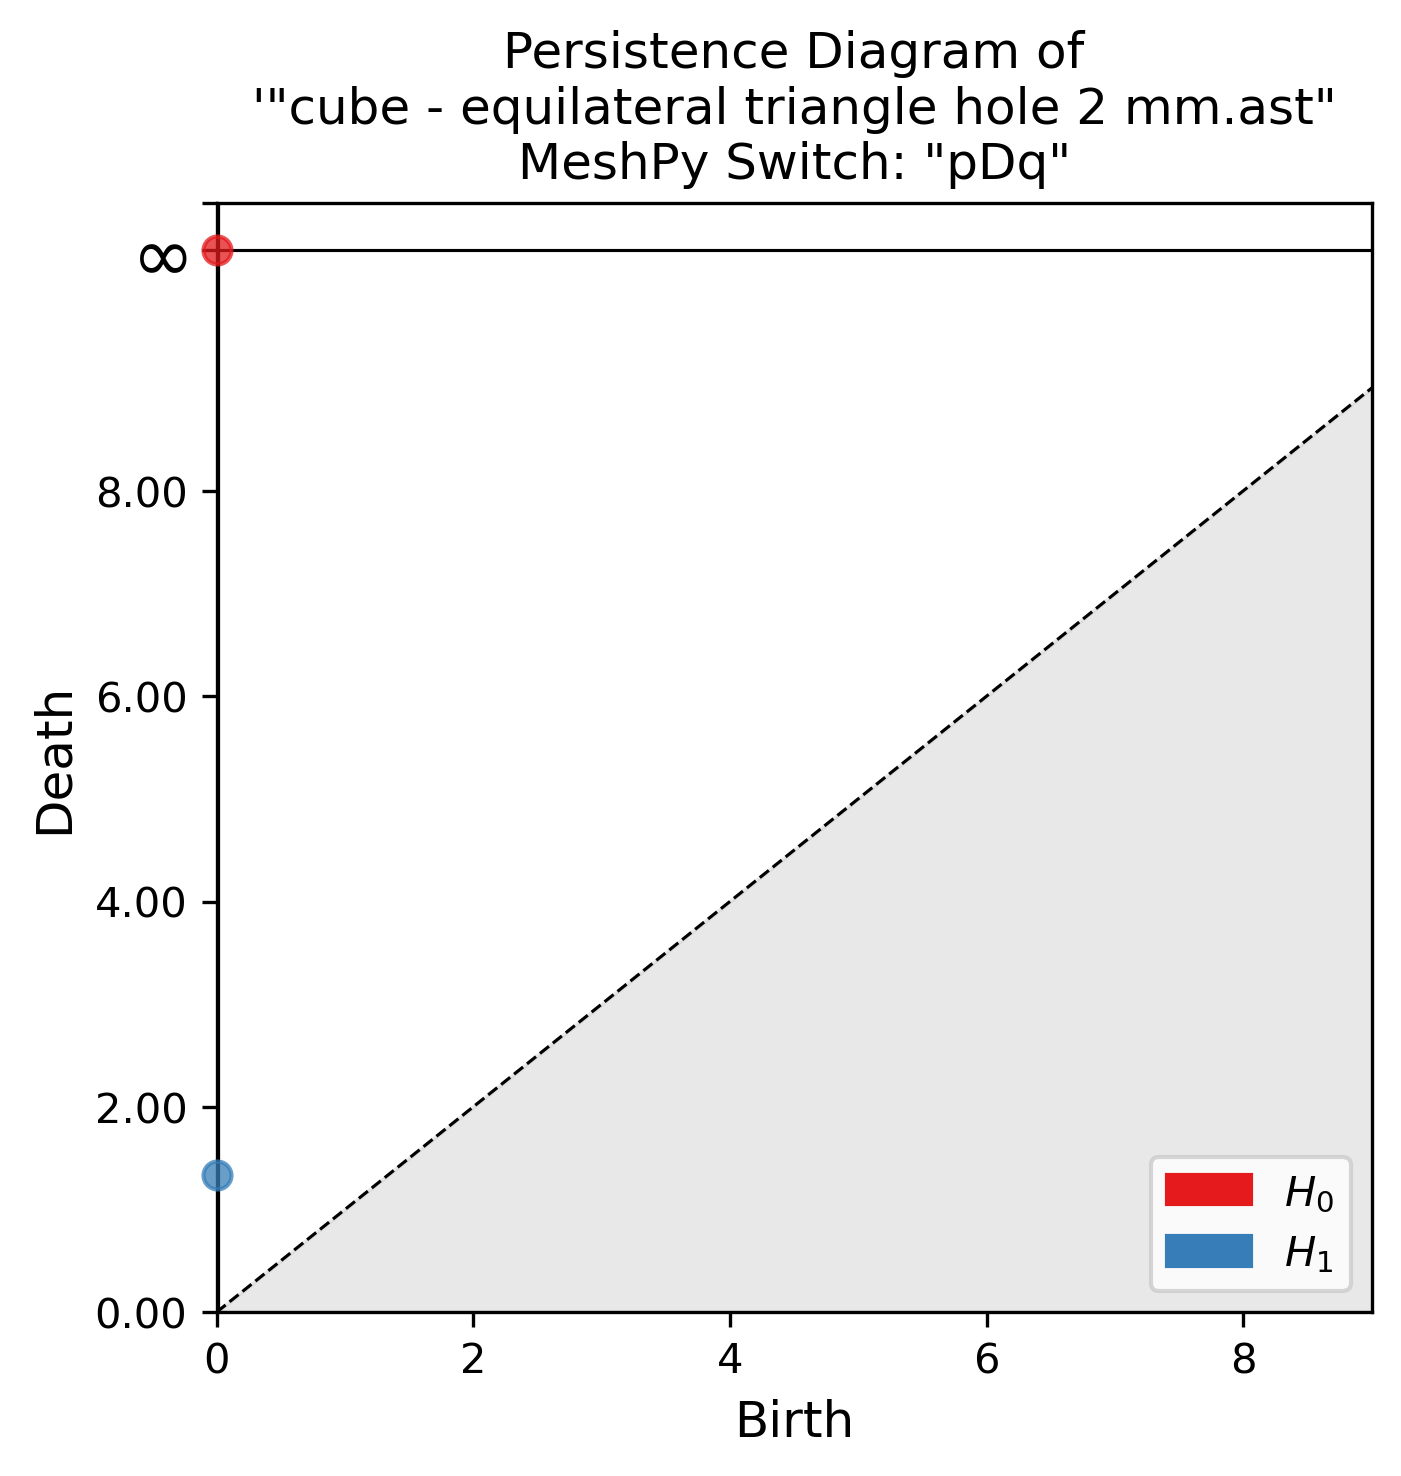
\includegraphics[width=2in]{Final Run, (cube - equilateral triangle hole 2 mm) persdia.svg} & 
         \includesvg[width=2in]{Final Run, (cube - equilateral triangle hole 1 mm) persdia.svg} & 
         \includegraphics[width=2in]{Final Run, (cube - equilateral triangle hole 0 Final Run, (cube - equilateral triangle hole 0 mm) persdiamm) persdia.svg} \\
         \hline
    \end{tabular}
    \caption{Persistence Diagrams of a rectangular prism ring with a cut that decreases to the original shape.}
    \label{fig:enter-label}
\end{figure}
\newpage
\begin{figure}
    \centering
    \begin{tabular}{|c|c|c|}
         \hline
         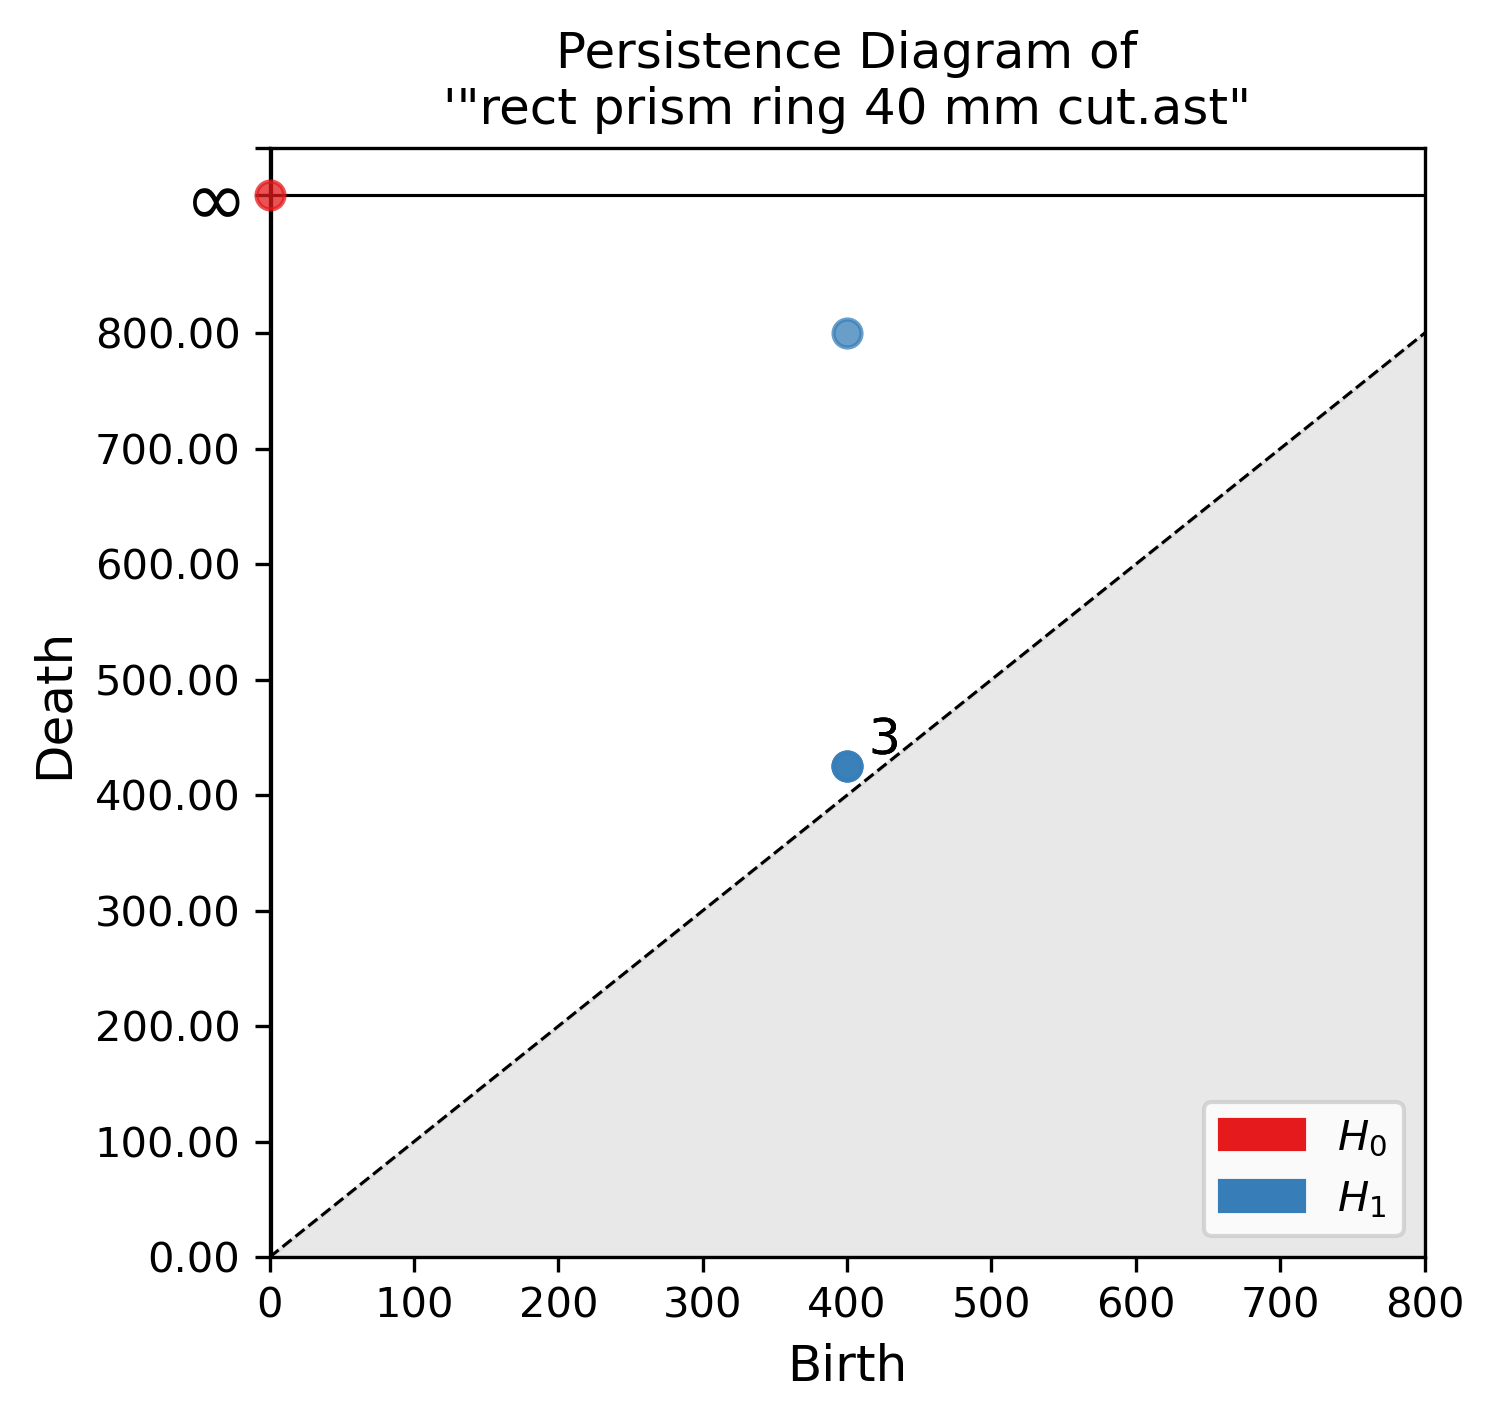
\includegraphics[width=2in]{Final Run, (rect prism ring 40 mm cut) persdia.svg} &
         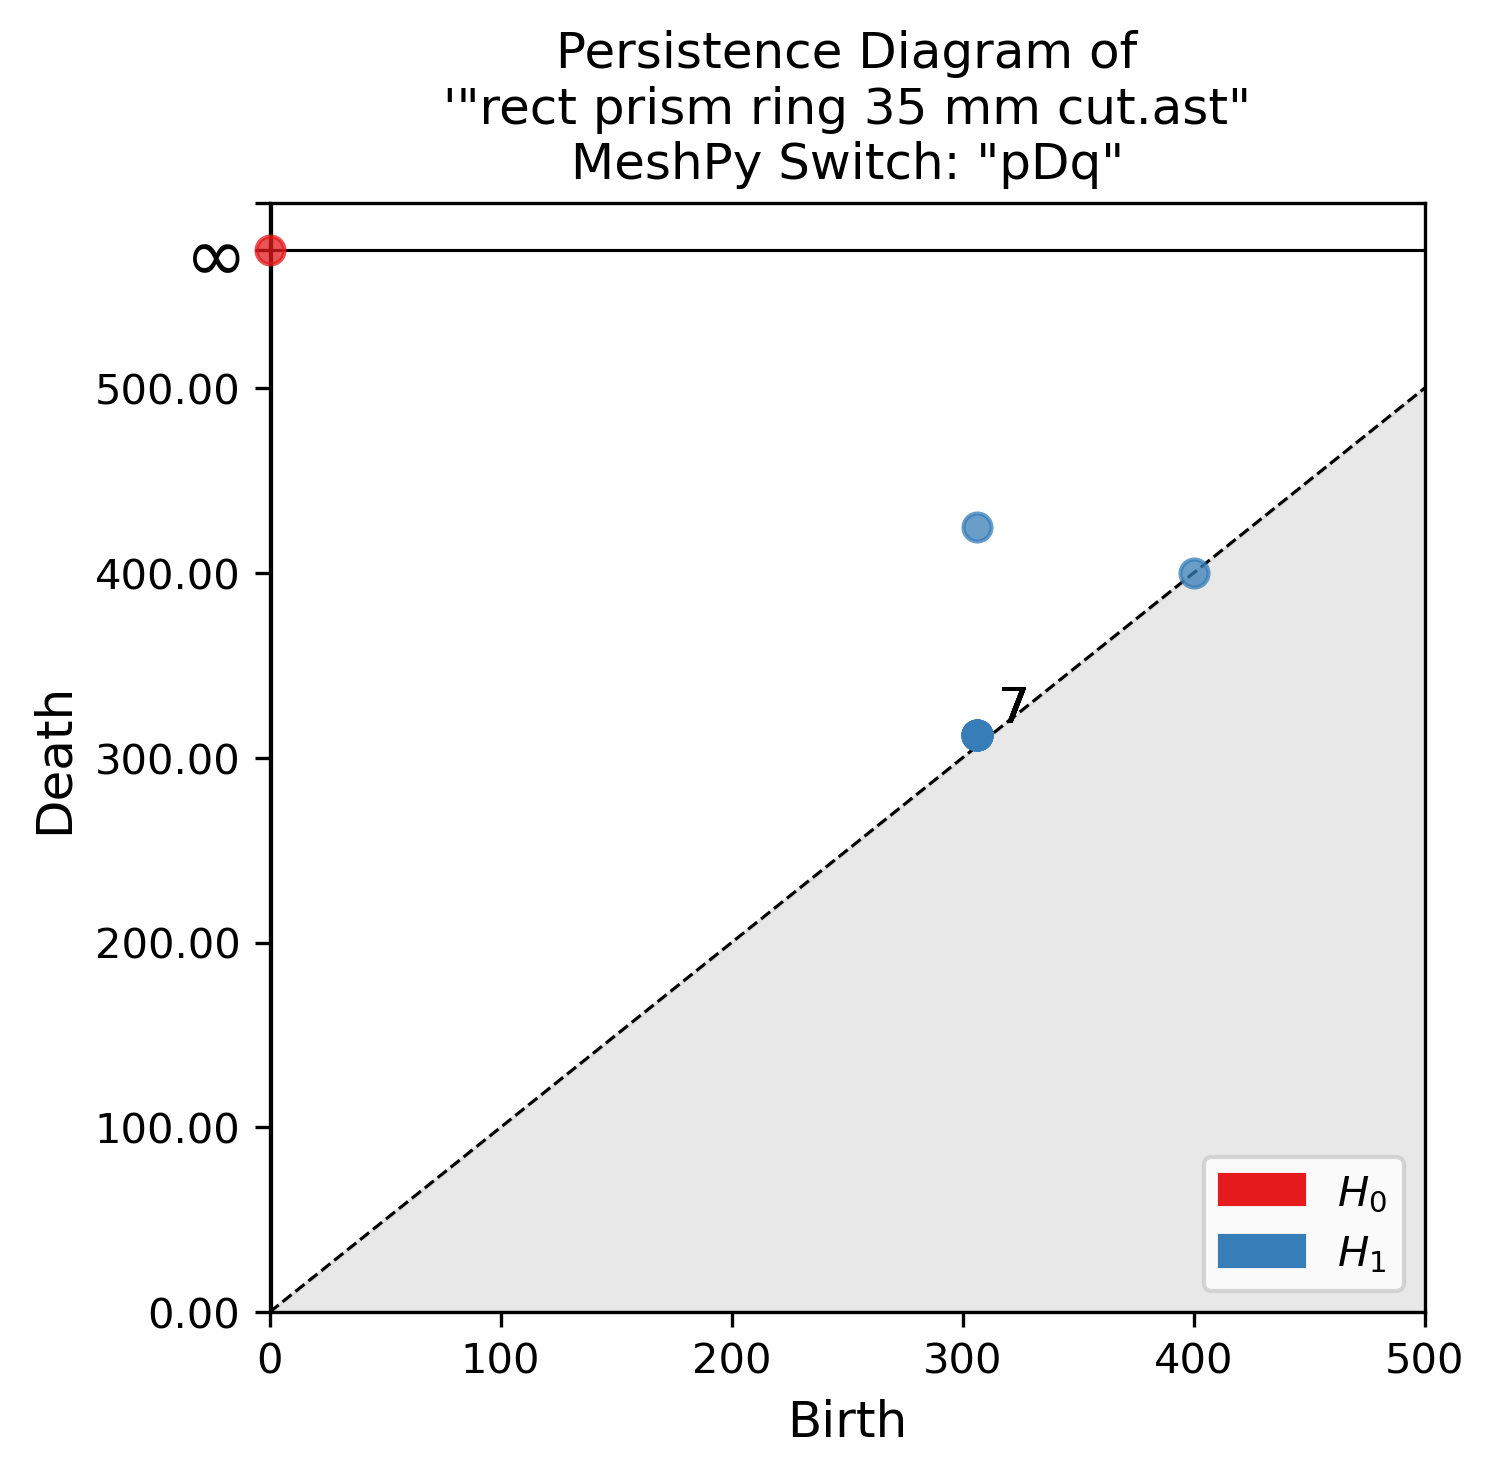
\includegraphics[width=2in]{Final Run, (rect prism ring 35 mm cut) persdia.svg} &  
         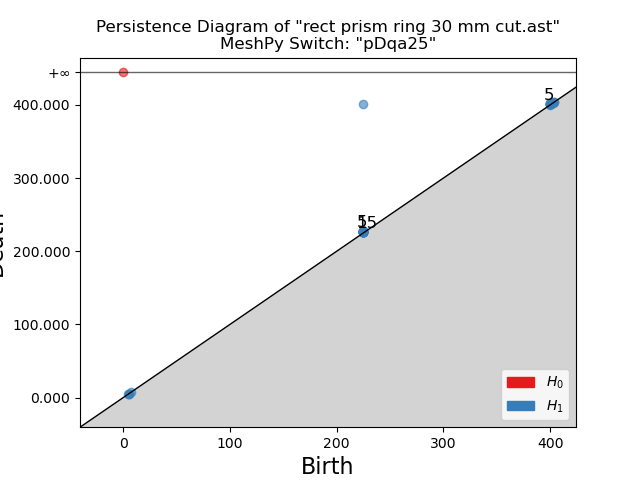
\includegraphics[width=2in]{Final Run, (rect prism ring 30 mm cut) persdia.svg} \\
         \hline
         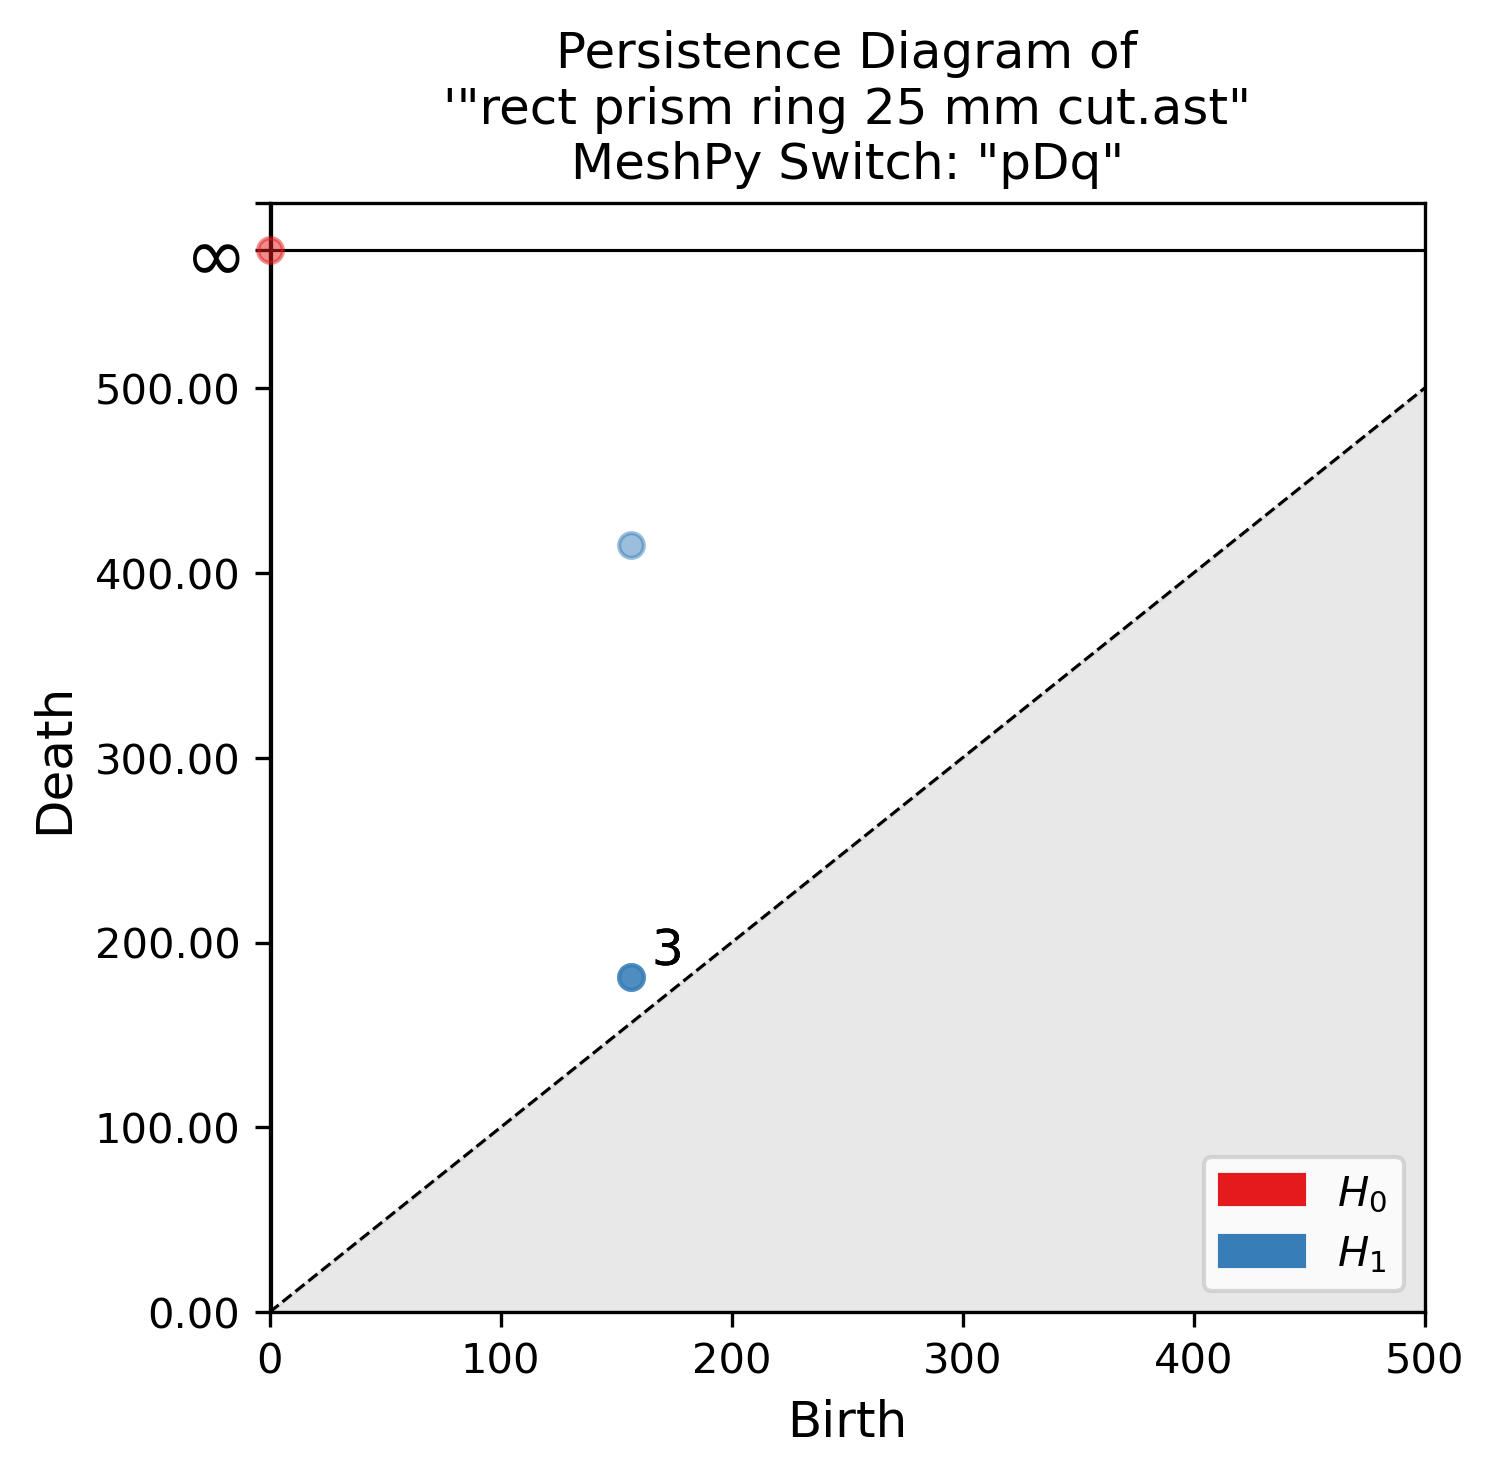
\includegraphics[width=2in]{Final Run, (rect prism ring 25 mm cut) persdia.svg} & 
         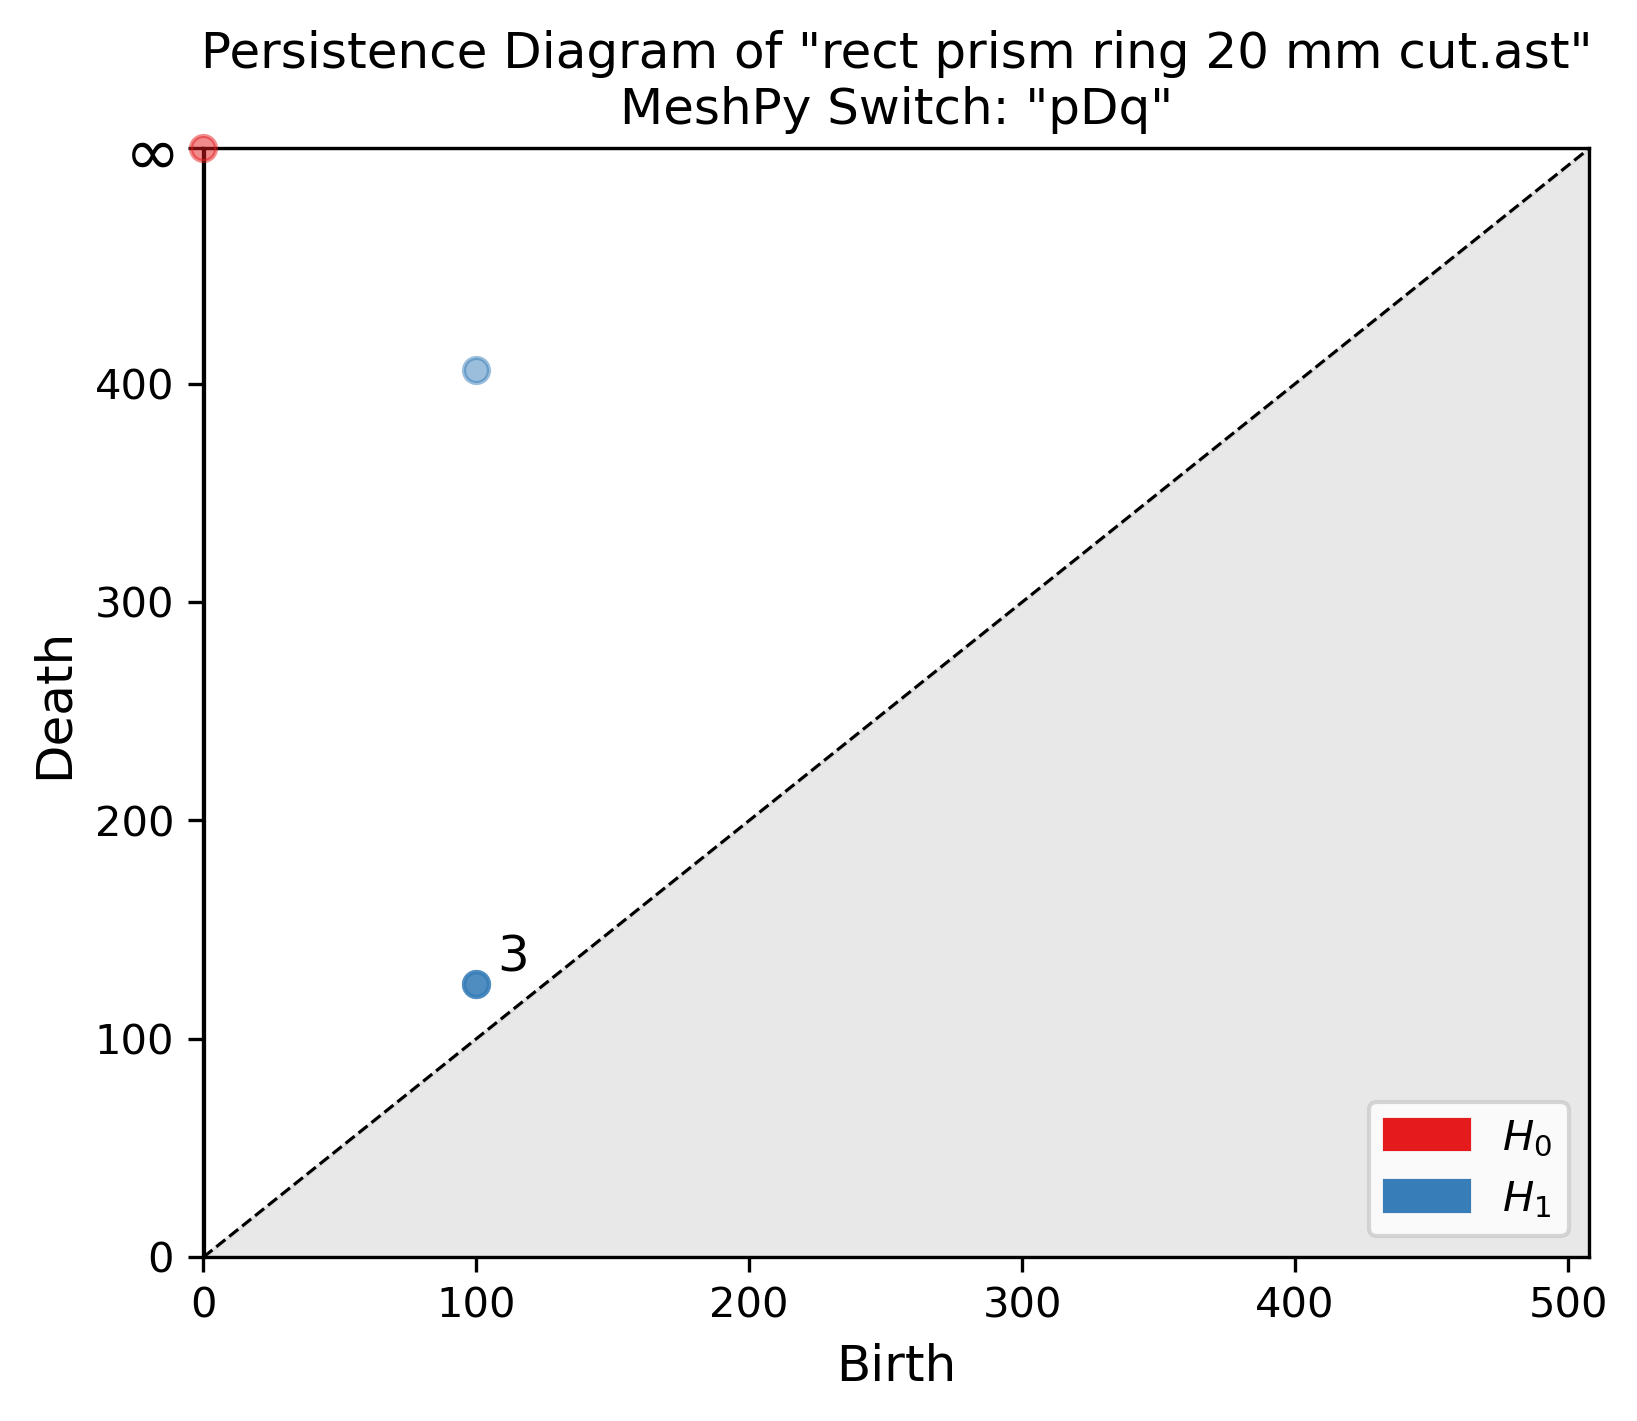
\includegraphics[width=2in]{Final Run, (rect prism ring 20 mm cut) persdia.svg} & 
         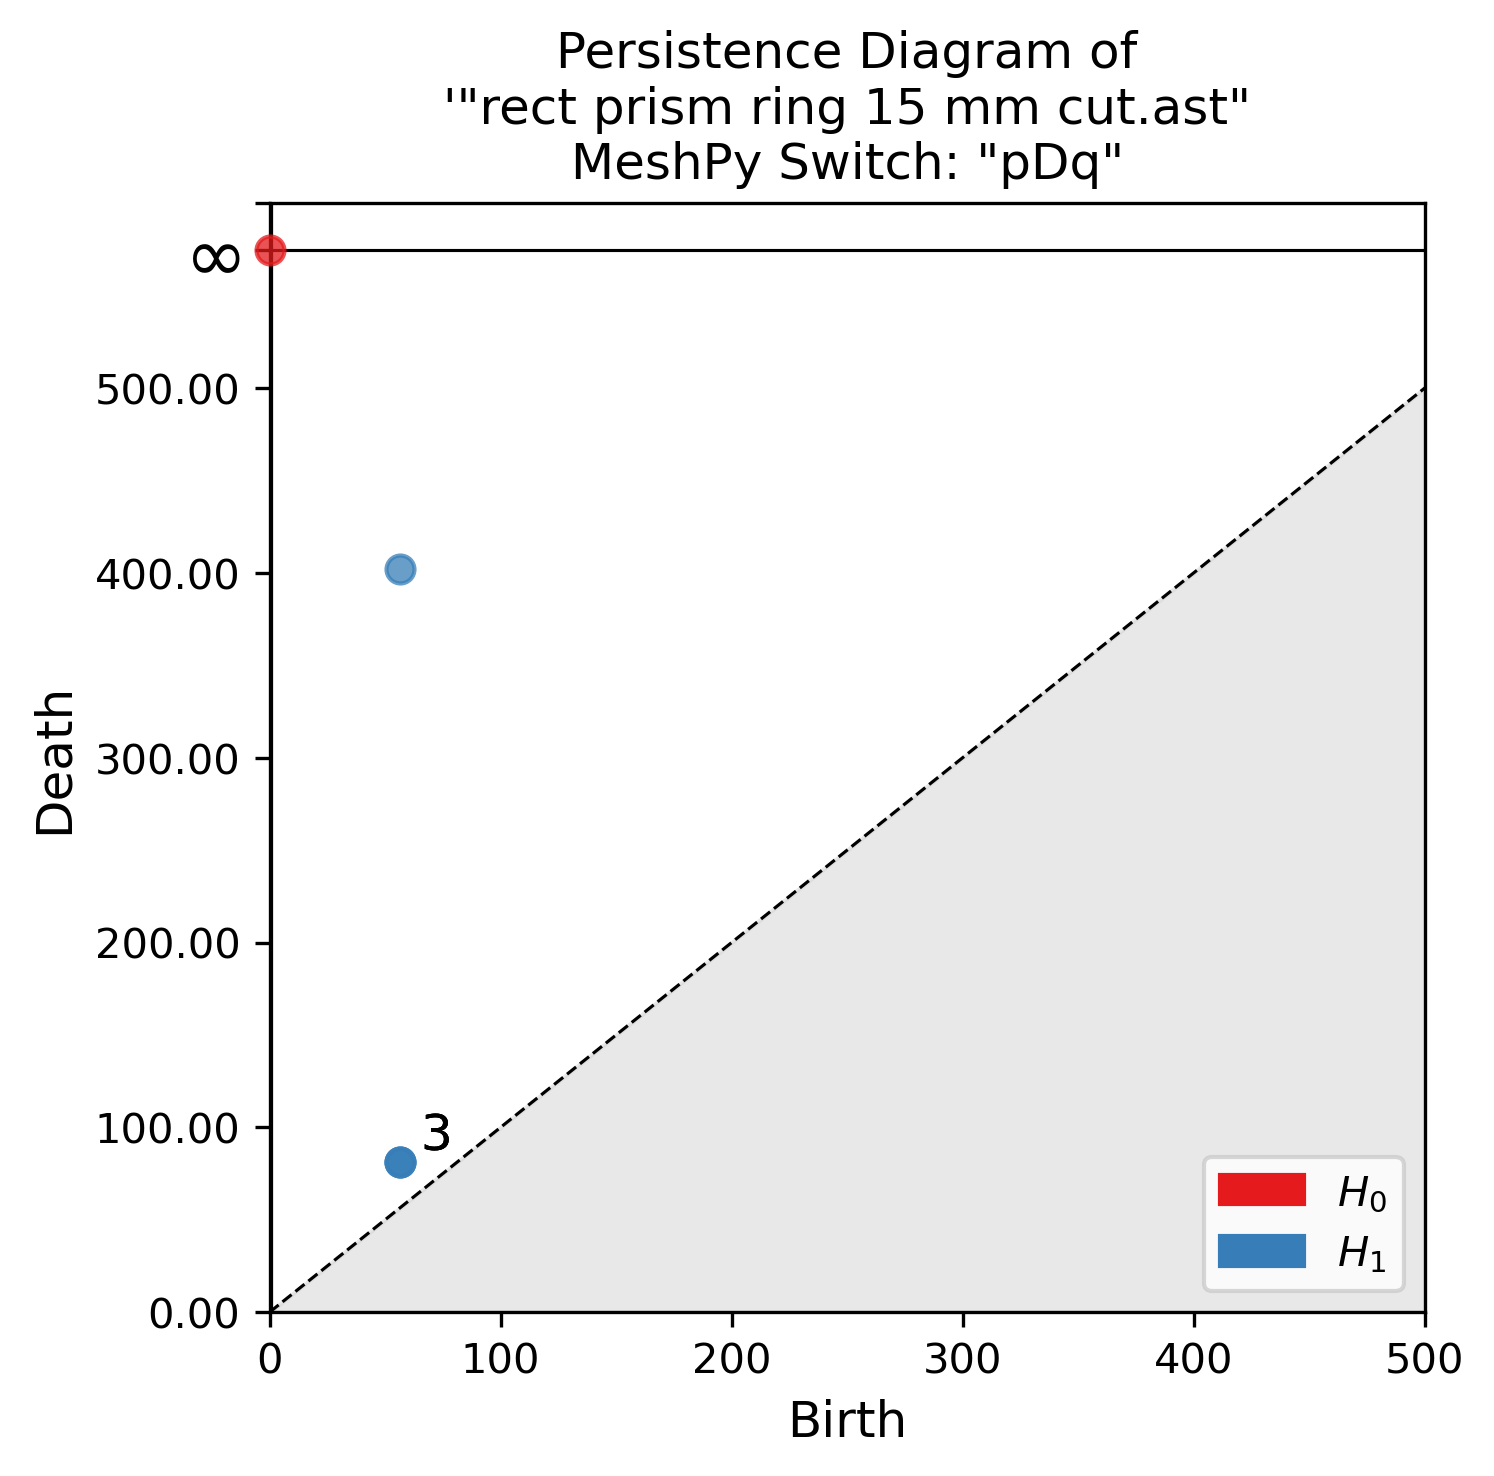
\includegraphics[width=2in]{Final Run, (rect prism ring 15 mm cut) persdia.svg} \\
         \hline
         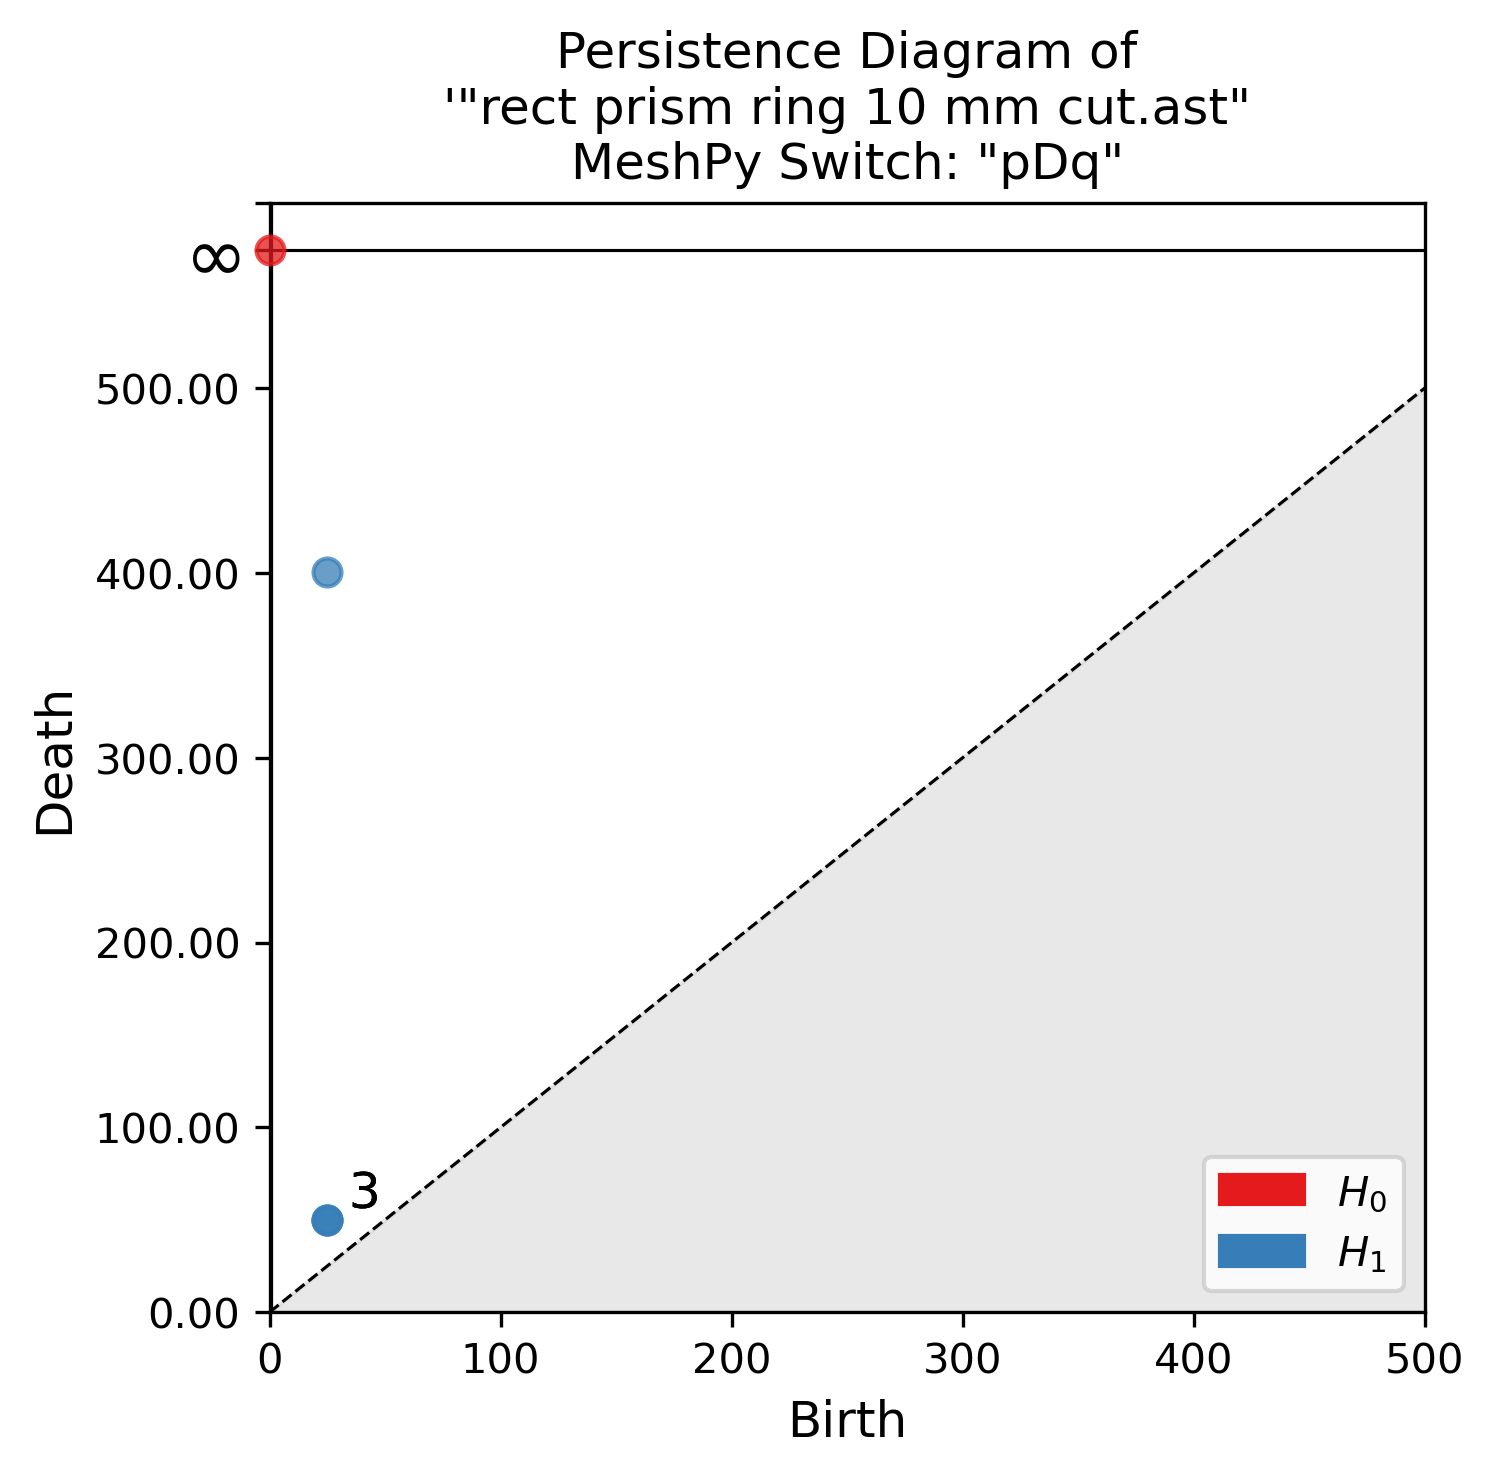
\includegraphics[width=2in]{Final Run, (rect prism ring 10 mm cut) persdia.svg} & 
         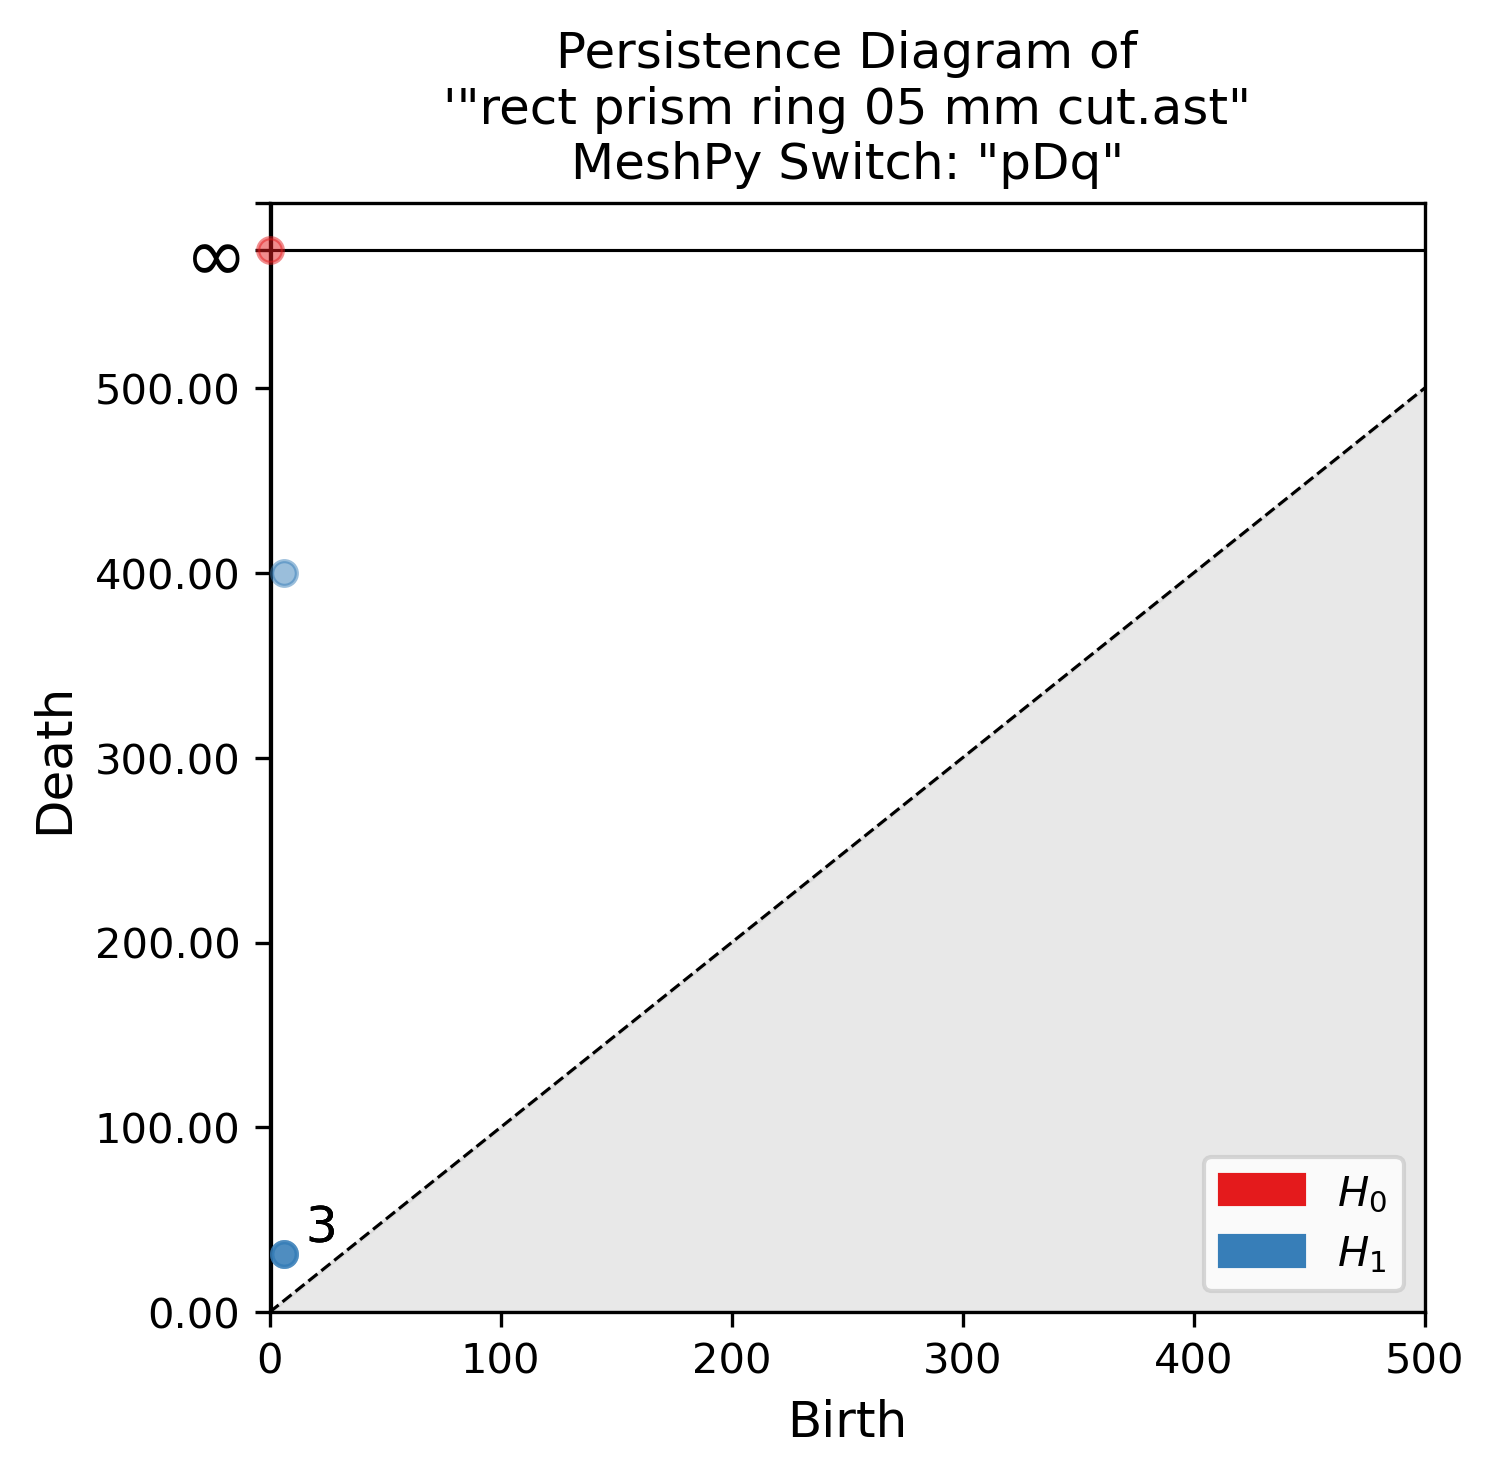
\includegraphics[width=2in]{Final Run, (rect prism ring 05 mm cut) persdia.svg} & 
         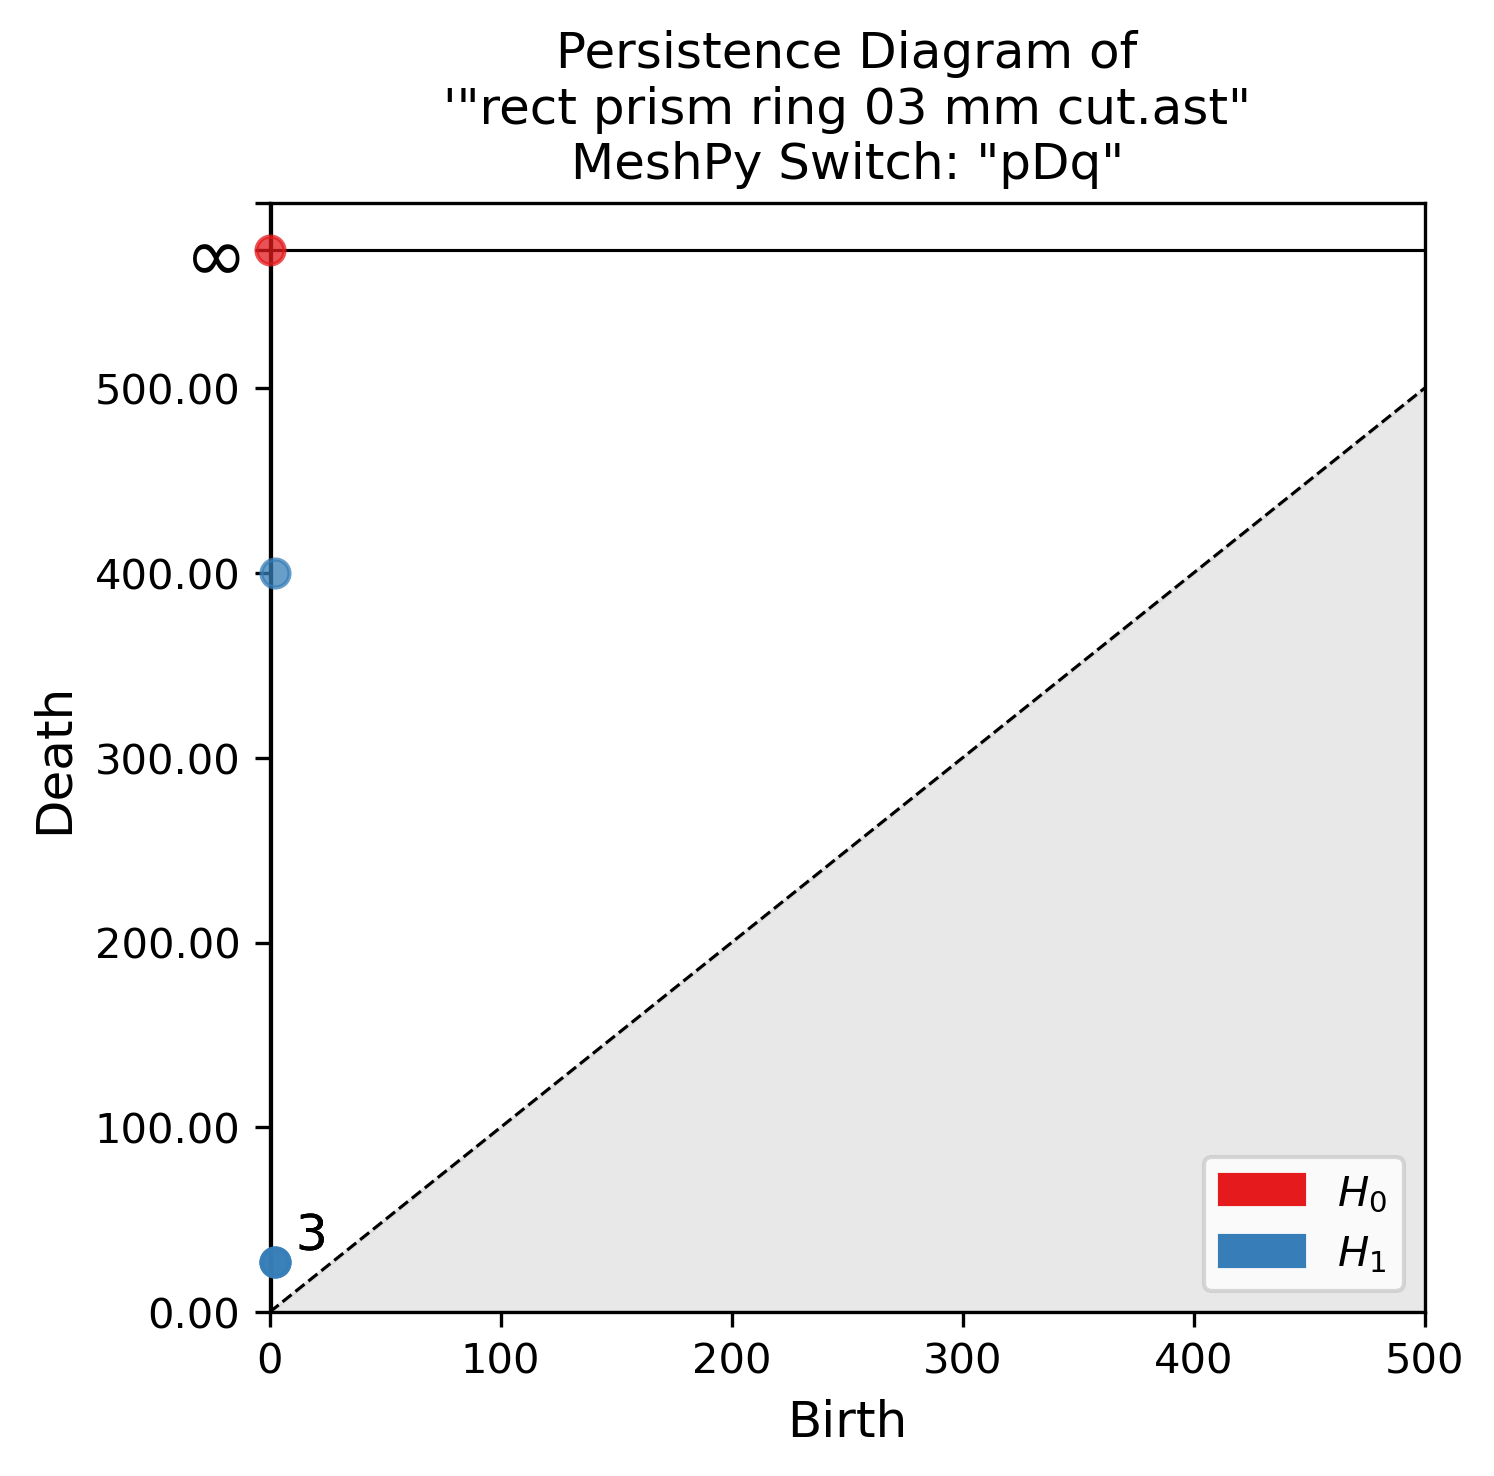
\includegraphics[width=2in]{Final Run, (rect prism ring 03 mm cut) persdia.svg} \\
         \hline
         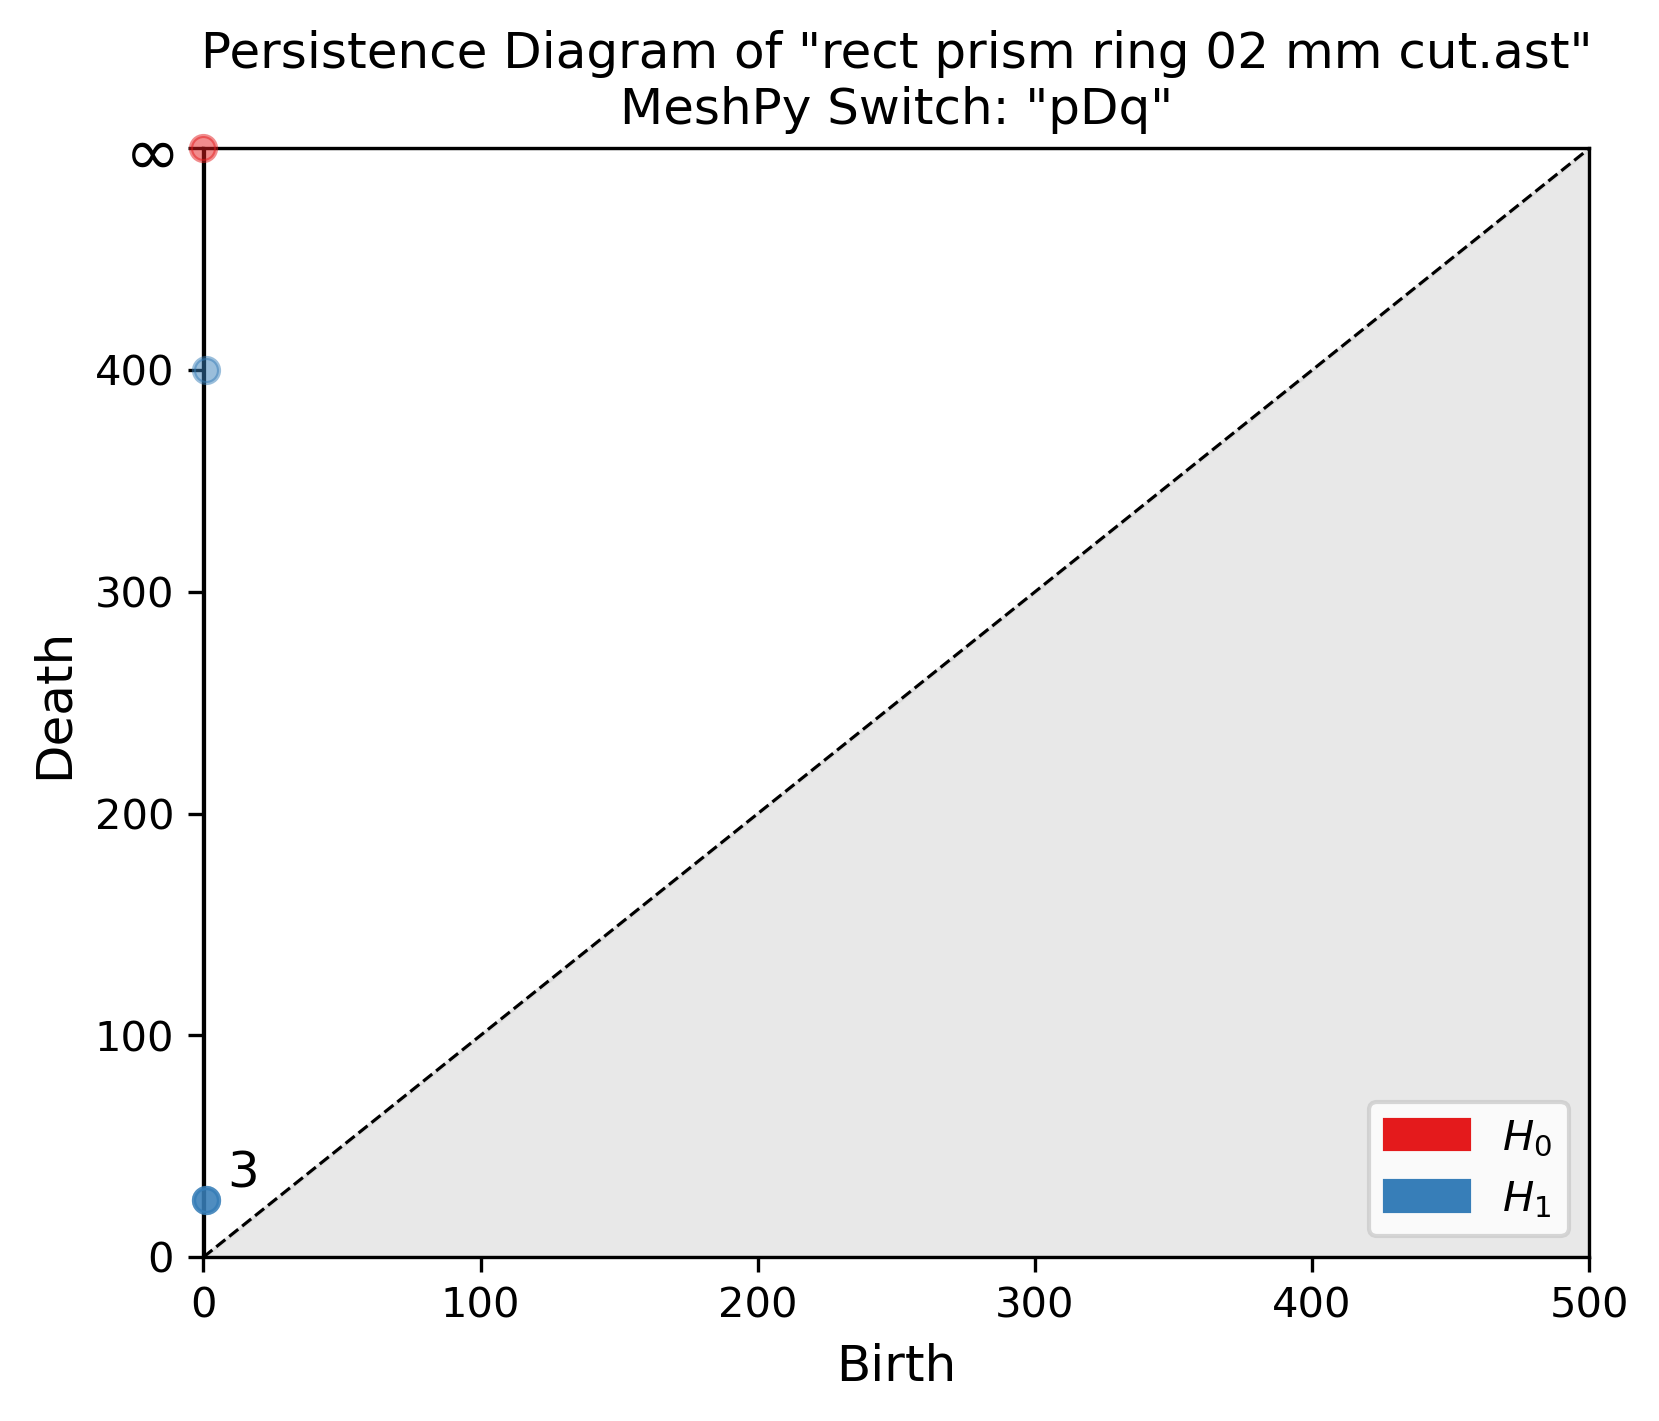
\includegraphics[width=2in]{Final Run, (rect prism ring 02 mm cut) persdia.svg} &
         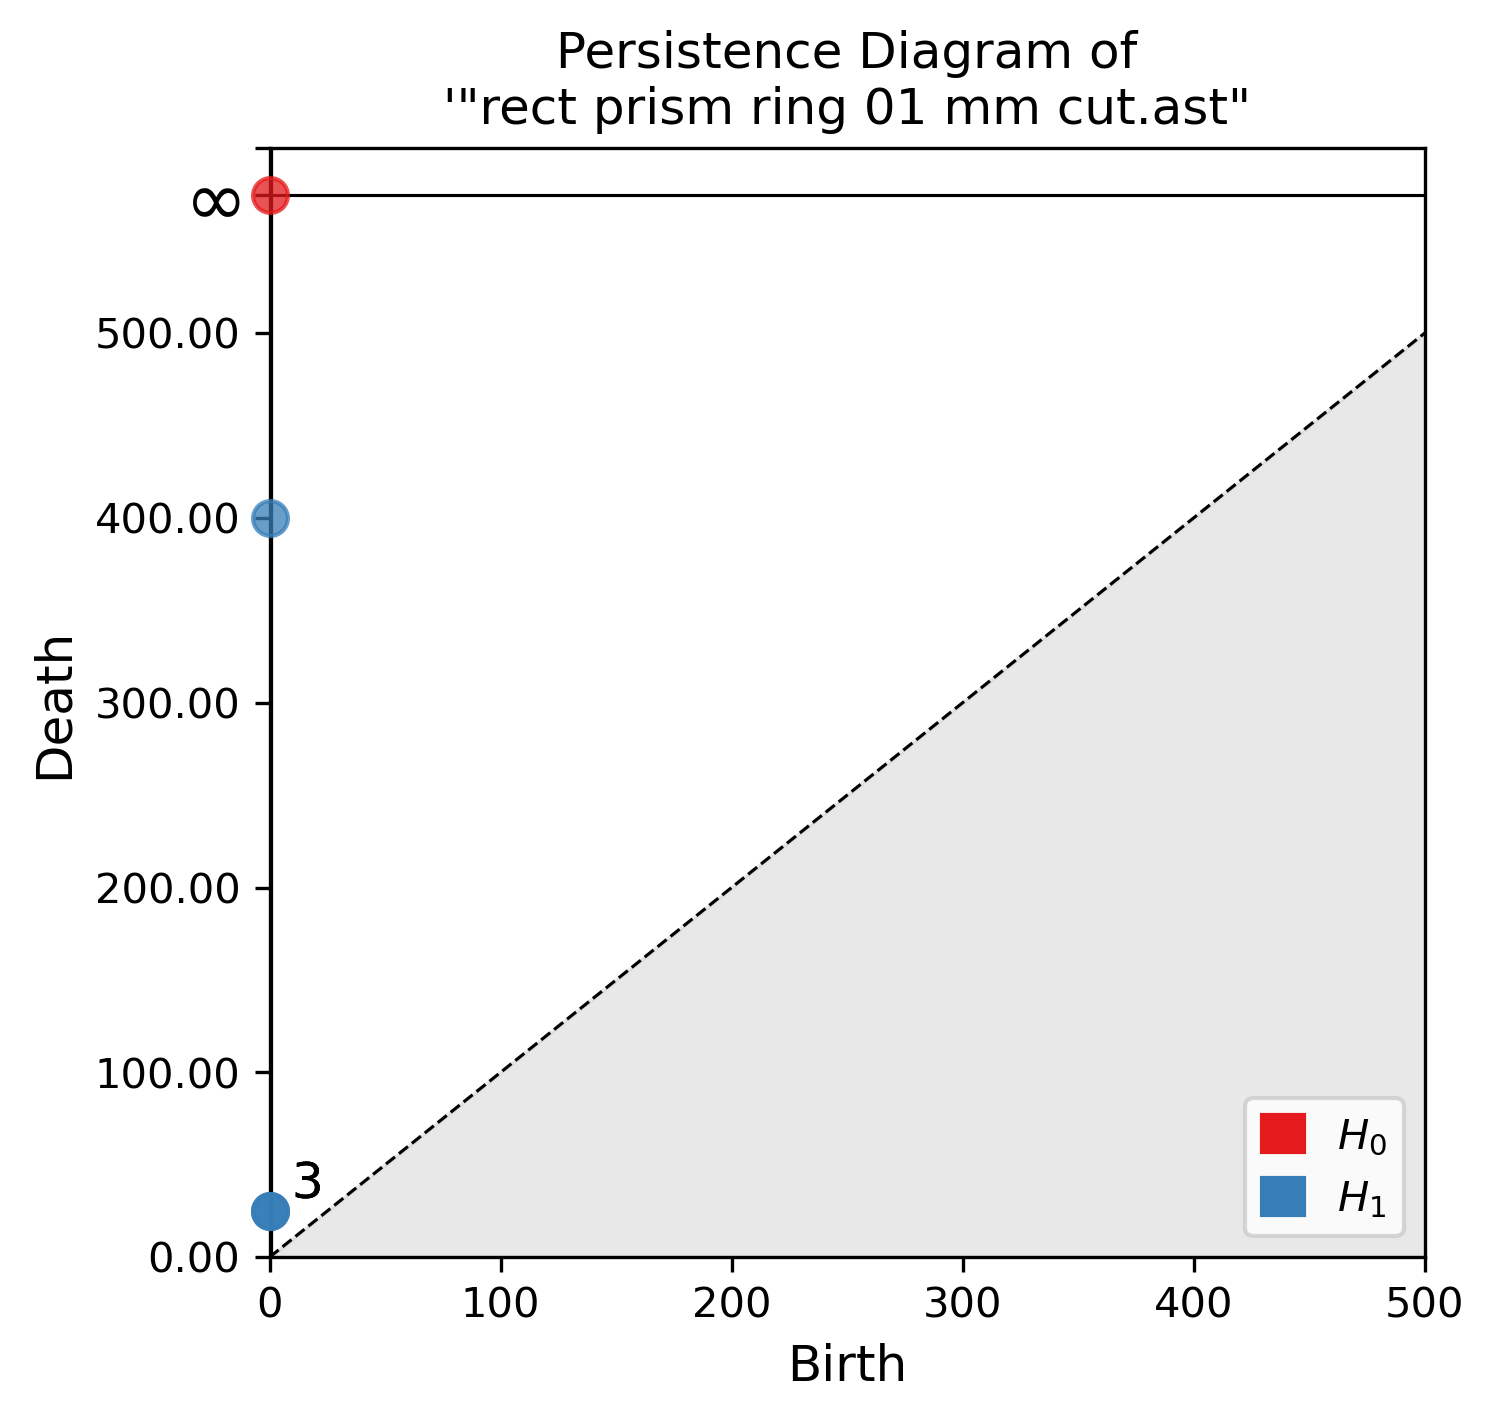
\includegraphics[width=2in]{Final Run, (rect prism ring 01 mm cut) persdia.svg} &
         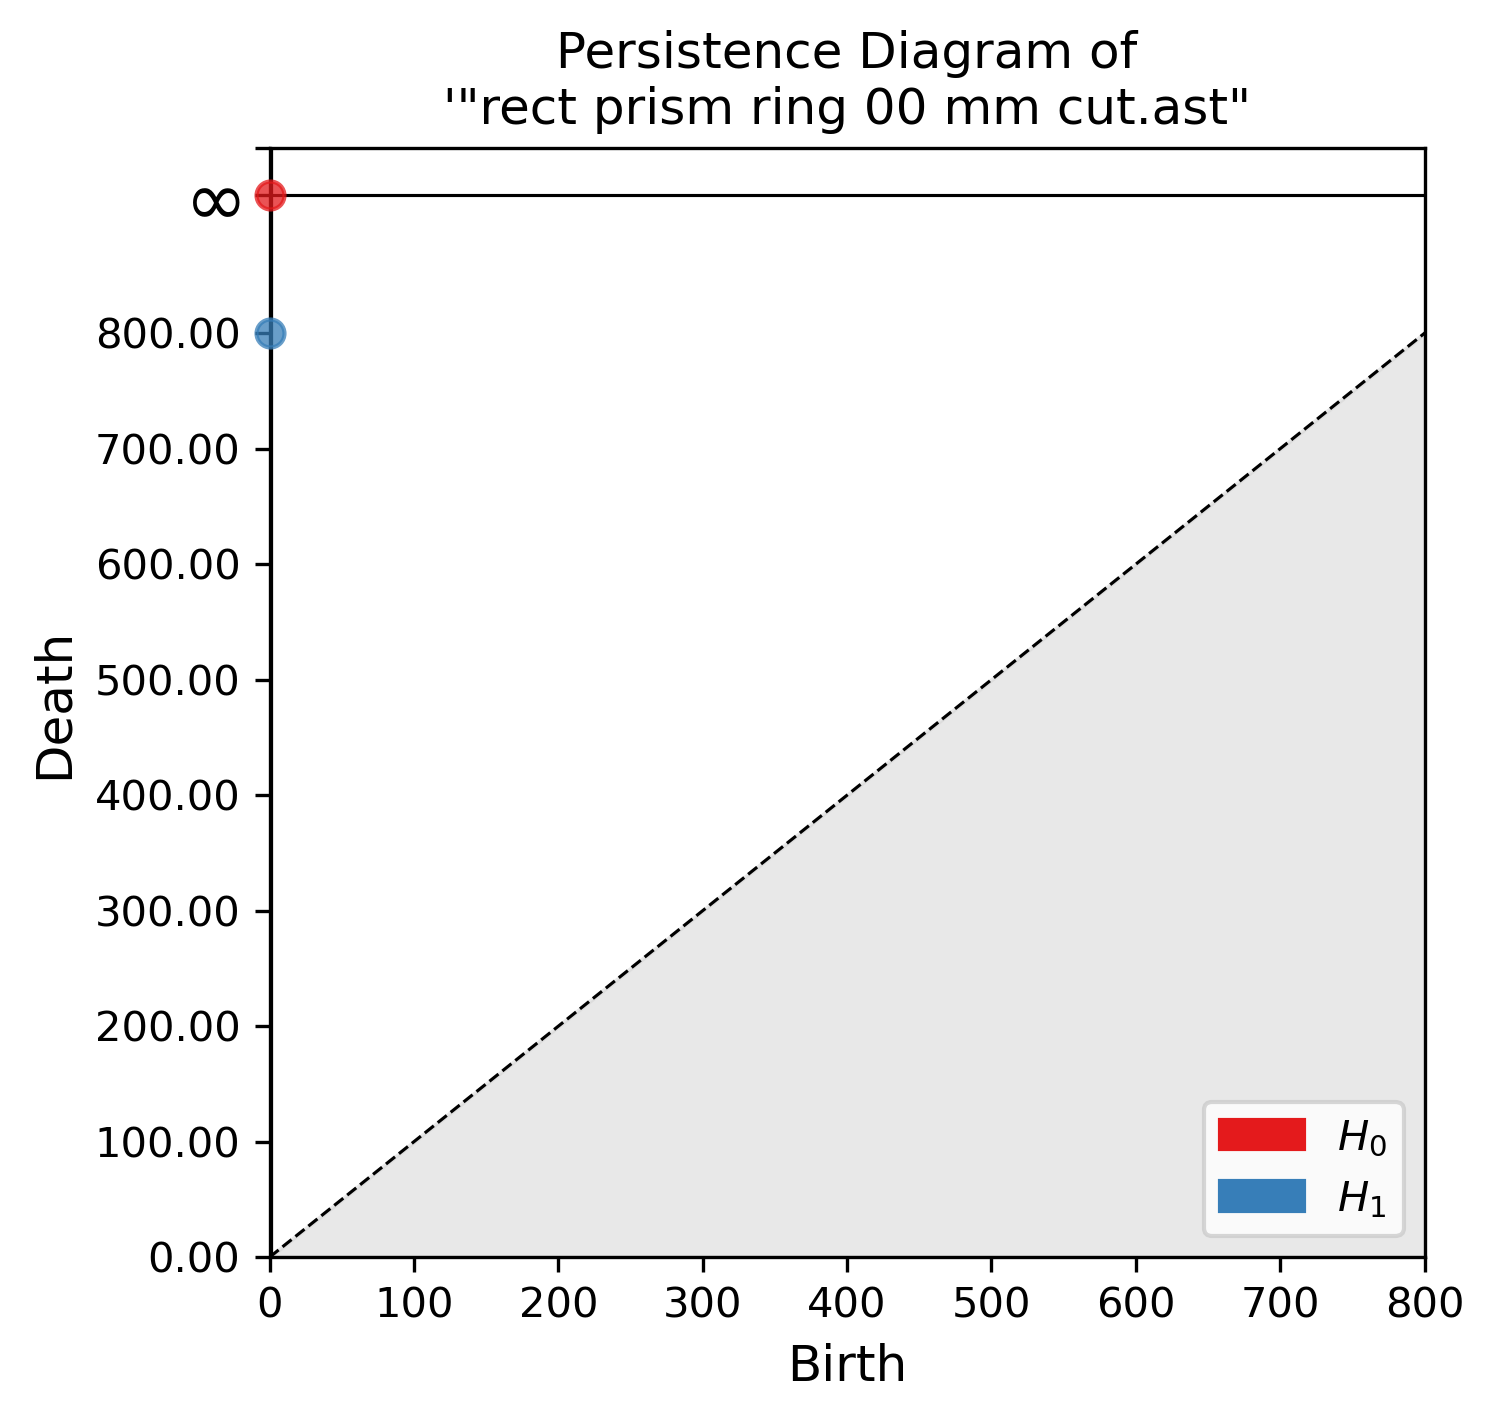
\includegraphics[width=2in]{Final Run, (rect prism ring 00 mm cut) persdia.svg} \\
         \hline
    \end{tabular}
    \caption{Persistence Diagrams of a rectangular prism ring with a cut that decreases to the original shape.}
    \label{fig:enter-label}
\end{figure}


\chapter{Discussion}

%%------------------------------------------------------------------%%
%%------------------------ Bibliography ----------------------------%%
%%------------------------------------------------------------------%%
%% Replace the myreferences with the name of your bib file.  Then you
%% can run bibtex as usual.
%%------------------------------------------------------------------%%


\bibliography{myreferences}
\bibliographystyle{plain}

%%------------------------------------------------------------------%%
%%------------------------- Appendices -----------------------------%%
%%------------------------------------------------------------------%%
%% If you choose not to have appendices, comment out the \appendix
%% line and the chapters below.
%%------------------------------------------------------------------%%
\appendix
\chapter{Appendix}

%%------------------------------------------------------------------%%
\backmatter
%%------------------------------------------------------------------%%
%%----------------------- YOU ARE FINISHED ! -----------------------%%
%%------------------------------------------------------------------%%
\end{document}
